\documentclass[12pt]{article}
\usepackage{import}
\input{/Users/henrytwiss/Documents/Documents/LaTeX/Vignettes/preamble.tex}

%=================%
%  Title & Index  %
%=================%
\title{Analytic \(L\)-functions}
\author{Henry Twiss}
\makeindex

\begin{document}
  \date{}
  \maketitle
  Throughout, \(s = \s+it\) and \(u = \tau+ir\) will stand for complex variables with \(\s\), \(\tau\), \(t\), and \(r\) real.
  \section{Analytic Data}
    An \textit{analytic \(L\)-function} \(L(s)\) is a Dirichlet series
    \[
      L(s) = \sum_{n \ge 1}\frac{a_{L}(n)}{n^{s}},
    \]
    with coefficients \(a_{L}(n) \in \C\) such that \(a_{L}(1) = 1\) and satisfying the following properties:
    \begin{enumerate}[align=left]
      \item[\textbf{Analyticity:}] There exists a nonnegative integer \(r_{L}\) such that the Dirichlet series of \(L(s)\) is absolutely convergent for \(\s > 1\) and admits meromorphic continuation to \(\C\) with at most a pole at \(s = 1\) of order \(r_{L}\). Moreover, \((s-1)^{r_{L}}L(s)\) is order \(1\).
      \item[\textbf{Functional Equation:}] There is a positive integer \(q_{L}\), called the \textit{conductor} of \(L(s)\), a positive integer \(d_{L}\) called the \textit{degree} of \(L(s)\), complex numbers \((\mu_{j})_{1 \le j \le d_{L}}\) called the \textit{local parameters} of \(L(s)\) at infinity that are either real or occur in conjugate pairs and satisfy \(\Re(\mu_{j}) \ge 0\), and a complex number \(\e_{L}\) called the \textit{root number} of \(L(s)\) with \(|\e_{L}| = 1\), all of which determine functions
      \[
        \L(s) = q_{L}^{\frac{s}{2}}L_{\infty}(s)L(s) \quad \text{and} \quad L_{\infty}(s) = \pi^{-\frac{d_{L}s}{2}}\prod_{j}\G\left(\frac{s+\mu_{j}}{2}\right),
      \]
      called the \textit{completion} of \(L(s)\) and the \textit{local factor} of \(L(s)\) at infinity respectively, satisfying
      \[
        \L(s) = \e_{L}\conj{\L(1-\conj{s})}.
      \]
      This is called the \textit{functional equation} of \(L(s)\). The tuple \((\e_{L},q_{L},\mu_{1},\ldots,\mu_{d_{L}})\) is called the \textit{functional equation data} of \(L(s)\). If \(p \mid q_{L}\) we say \(p\) is \textit{ramified} while if \(p \nmid q_{L}\) we say \(p\) is \textit{unramified}.
      \item[\textbf{Euler product:}] For every prime \(p\), there exist complex numbers \((\a_{j}(p))_{1 \le j \le d_{L}}\) called the \textit{local parameters} of \(L(s)\) at \(p\) satisfying \(|\a_{j}(p)| < p\) and are such that \(L(s)\) admits the Euler product
      \[
        L(s) = \prod_{p}(1-\a_{1}(p)p^{-s})^{-1} \cdots (1-\a_{d_{L}}(p)p^{-s})^{-1},
      \]
      which is absolutely convergent for \(\s > 1\). The polynomial \(L_{p}\) defined by
      \[
        L_{p}(T) = (1-\a_{1}(p)T) \cdots (1-\a_{d_{L}}(p)T),
      \]
      is called the \textit{local factor} of \(L(s)\) at \(p\). If \(p\) is unramified then \(L_{p}\) is of degree \(d_{L}\) while if \(p\) is ramified then \(L_{p}\) is of degree less than \(d_{L}\).
    \end{enumerate}

    An analytic \(L\)-function is said to be \textit{unitary} if it satisfies the following two additional properties:

    \begin{enumerate}[align=left]
      \item[\textbf{Selberg bound:}] The local parameters at infinity satisfy \(\Re(\mu_{j}) \in \frac{1}{2}\Z_{\ge 0}\).
      \item[\textbf{Ramanujan bound:}] The local parameters at \(p\) satisfy \(|\a_{j}(p)| = 1\) for unramified \(p\) and \(|\a_{j}(p)| \le 1\) for ramified \(p\).
    \end{enumerate}

    Some comments on the definition of analytic \(L\)-functions are in order.
    \begin{enumerate}[label*=(\roman*)]
      \item The bound \(\Re(\mu_{j}) \ge 0\) ensures that the local factor at infinity is holomorphic in the region \(\s > 0\). As this factor is then guaranteed to be finite and nonzero at \(s = 1\), the completion possesses a pole at \(s = 1\) of order \(r\). By the functional equation, the completion also has a pole at \(s = 0\) of the same order.
      \item If we merely assume \((s-1)^{r_{L}}L(s)\) is finite order then the functional equation forces the order to be \(1\). This can be deduced by considering the entire function
    \[
      s^{r_{L}}(s-1)^{r_{L}}\L(s),
    \]
    and applying the Phragm\'en-Lindel\"of convexity principle in vertical strips.
    \item The condition that the root number satisfies \(|\e_{L}| = 1\) isn't strictly necessary. For applying the functional equation twice shows \(|\e_{L}|^{2} = 1\).
    \item As the gamma function is conjugation-equivariant and the local parameters at infinity are real or occur in conjugate pairs, the local factor at infinity is also conjugation-equivariant. This means that we can write the functional equation in the form
    \[
      q_{L}^{\frac{s}{2}}L_{\infty}(s)L(s) = \e_{L}q_{L}^{\frac{1-s}{2}}L_{\infty}(1-s)\conj{L(1-\conj{s})}.
    \]
    \item Most analytic \(L\)-functions are only conjectured to be unitary. In any case, the Ramanujan bound is the more important of the two. The Euler product implies that the coefficients \(a_{L}(n)\) are multiplicative and are determined on prime powers by
    \[
      a_{L}(p^{k}) = \sum_{1 \le j_{1} \le \cdots \le j_{k} \le d_{L}}\a_{j_{1}}(p) \cdots \a_{j_{k}}(p).
    \]
    In other words, \(a_{L}(p^{k})\) is the complete symmetric polynomial of degree \(k\) in the local parameters at \(p\) and there are \(\binom{k+d_{L}-1}{d_{L}-1} \ll \s_{d_{L}}(p^{k})\) many terms. If the Ramanujan bound holds, then it follows that \(a_{L}(n) \ll \s_{d_{L}}(n)\). This implies the slightly weaker, but more practical, estimate \(a_{L}(n) \ll_{\e} n^{\e}\).
    \end{enumerate}

    As \(L(s)\) is absolute convergent for \(\s > 1\) and admits an Euler product there, we can take the logarithm of the Euler product and differentiate termwise to compute the logarithmic derivative. A short computation shows
    \[
       -\frac{L'}{L}(s) = \sum_{n \ge 1}\frac{\L_{L}(n)}{n^{s}},
    \]
    is an absolutely convergent Dirichlet series for \(\s > 1\) where
    \[
      \L_{L}(n) = \begin{cases} \sum_{j}\a_{j}(p)^{k}\log(p) & \text{if \(n = p^{k}\)}, \\ 0 & \text{otherwise}. \end{cases}
    \]
    We call \(\L_{L}(n)\) the \textit{Von Mangoldt coefficient} of \(L(s)\).

    It it clear from the definition that analytic \(L\)-functions are closed under multiplication and that the degree is additive. Moreover, this closure respects unitary \(L\)-functions. This makes the set of analytic \(L\)-functions into a graded commutative semigroup where the grading is induced by degree. It follows that there exist irreducible elements with respect to the grading and we say that an analytic \(L\)-function is \textit{primitive} if it such an irreducible. Clearly any analytic \(L\)-function of degree \(1\) is primitive. Moreover, every analytic \(L\)-function factors into a product of primitive \(L\)-functions. Such a factorization is only conjectured to be unique for unitary \(L\)-functions. A sufficient condition would be \textit{Selberg's orthogonality conjecture}.

    \begin{conjecture*}[Selberg's orthogonality conjecture]
      For any two primitive unitary \(L\)-functions \(L_{1}(s)\) and \(L_{2}(s)\), we have
      \[
        \sum_{p \le x}\frac{a_{L_{1}}(p)\conj{a_{L_{2}}(p)}}{p} = \d_{L_{1},L_{2}}\log\log(x)+O(1).
      \]
    \end{conjecture*}

    Indeed, we have the following result:

    \begin{proposition}
      Assume Selberg's orthogonality conjecture. Then every unitary \(L\)-function factors uniquely into a product of primitive unitary \(L\)-functions.
    \end{proposition}
    \begin{proof}
      If the factorization into primitive unity \(L\)-functions were not unique, then we would have distinct factorizations satisfying
      \[
        L_{1}(s) \cdots L_{n}(s) = M_{1}(s) \cdots M_{m}(s),
      \]
      for some primitive unitary \(L\)-functions \(L_{i}\) and \(M_{j}\). By uniqueness of coefficients of Dirichlet series, compare the \(p\)-th coefficient to see that
      \[
        \sum_{i}a_{L_{i}}(p) = \sum_{j}a_{M_{j}}(p).
      \]
      Now consider
      \[
        \sum_{p < x}\frac{1}{p}\left(\sum_{i}a_{L_{i}}(p)\right)\left(\sum_{j}\conj{a_{M_{j}}(p)}\right) = \sum_{i,j}\sum_{p < x}\frac{a_{L_{i}}(p)\conj{a_{M_{j}}(p)}}{p}.
      \]
      Selberg's orthogonality conjecture implies
      \[
        O(1) = c\log\log(x)+O(1),
      \]
      for some positive integer \(c\) since the factorizations are distinct. This is impossible.
    \end{proof}

    To an analytic \(L\)-function, we also associate its \textit{analytic conductor} \(\mf{q}(s)\) defined by
    \[
      \mf{q}(s) = q_{L}\mf{q}_{\infty}(s),
    \]
    where
    \[
      \mf{q}_{\infty}(s) = \prod_{j}(|s+\mu_{j}|+3).
    \]
    The choice of \(3\) in \(|s+\mu_{j}|+3\) is a matter of convenience as could use any positive constant. In particular, it is useful when taking logarithms as \(\log(|s+\mu_{j}|+3) \ge 1\). For legibility, we write also write
    \[
      \mf{q} = \mf{q}(0) \quad \text{and} \quad \mf{q}_{\infty} = \mf{q}_{\infty}(0).
    \]
    Estimates for the analytic conductor follow from those of the gamma function. Recall from Stirling's formula that
    \[
      \frac{\G(1-s)}{\G(s)} \ll_{\e} (|t|+3)^{1-2\s},
    \]
    provided \(\s_{1} \le \s \le \s_{2}\) and \(s\) is at least distance \(\e\) away from the poles of the gamma function. Then the estimates
     \begin{equation}\label{equ:gamma_factor_analytic_conductor_estimate}
      \frac{L_{\infty}(1-s)}{L_{\infty}(s)} \ll_{\e} \mf{q}_{\infty}(s)^{\frac{1}{2}-\s} \quad \text{and} \quad q_{L}^{\frac{1}{2}-s}\frac{L_{\infty}(1-s)}{L_{\infty}(s)} \ll_{\e} \mf{q}(s)^{\frac{1}{2}-\s},
    \end{equation}
    in the same region. An associated estimate can be obtain for the logarithmic derivative of the analytic conductor. Recall from the logarithm of Stirling's formula that
    \[
      \frac{\G'}{\G}(s) \ll \log(|s|+3),
    \]
    provided \(\s_{1} \le \s \le \s_{2}\) and \(s\) is at least distance \(\e\) away from the poles of the gamma function. Then the estimates
    \begin{equation}\label{equ:digamma_gamma_factor_analytic_conductor_estimate}
      \frac{L_{\infty}'}{L_{\infty}}(s) \ll_{\e} \log\mf{q}_{\infty}(s) \quad \text{and} \quad \log{q_{L}}+\frac{L_{\infty}'}{L_{\infty}}(s) \ll_{\e} \log\mf{q}(s),
    \end{equation}
    are valid in the same region.

    The \textit{critical strip} of an analytic \(L\)-function is the vertical strip left invariant by the transformation \(s \mapsto 1-s\). This is the region defined by
    \[
      \left\{s \in \C:\left|\s-\frac{1}{2}\right| \le \frac{1}{2}\right\}.
    \]

    \begin{figure}[ht]
      \centering
      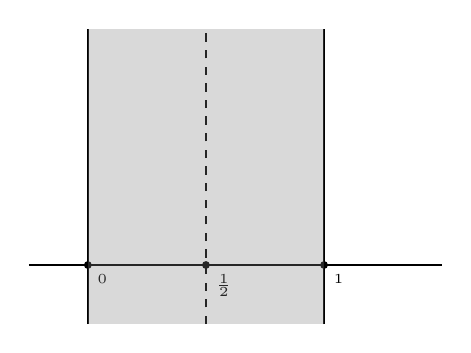
\begin{tikzpicture}[scale=1.5]
        \def\xmin{-0.5} \def\xmax{3}
        \def\ymin{-0.5} \def\ymax{2}
        \draw[thick] (\xmin,0) -- (\xmax,0);
        \draw[thick] (0,\ymin) -- (0,\ymax);
        \draw[thick] (2,\ymin) -- (2,\ymax);
        \draw[dashed] (1,\ymin) -- (1,\ymax);

        \node at (0,0) [below right] {\tiny{\(0\)}};
        \node at (0,0) [circle,fill,inner sep=1pt]{};
        \node at (1,0) [below right] {\tiny{\(\frac{1}{2}\)}};
        \node at (1,0) [circle,fill,inner sep=1pt]{};
        \node at (2,0) [below right] {\tiny{\(1\)}};
        \node at (2,0) [circle,fill,inner sep=1pt]{};

        \begin{scope}
          \path[clip] (0,\ymin) -- (0,\ymax) -- (2,\ymax) -- (2,\ymin) -- cycle;
          \fill[gray,opacity=0.3] (0,\ymin) rectangle (2,\ymax);
        \end{scope}
      \end{tikzpicture}
      \caption{The critical strip.}
      \label{fig:critical_strip}
    \end{figure}

    The \textit{critical line} is the line left invariant by the transformation \(s \mapsto 1-s\) which is also given by \(\s = \frac{1}{2}\). The critical line bisects the critical strip vertically. The \textit{central point} is the fixed point of the transformation \(s \mapsto 1-s\), in other words, the point \(s = \frac{1}{2}\). Clearly the central point is also the center of the critical line. The critical strip, critical line, and central point are all displayed in \cref{fig:critical_strip}.

    In the region \(\s > 1\) we may study the analytic properties of \(L(s)\) via its Dirichlet series. Using the functional equation, we may write
    \[
      L(s) = \e_{L}q_{L}^{\frac{1}{2}-s}\frac{L_{\infty}(1-s)}{L_{\infty}(s)}\conj{L(1-\conj{s})}.
    \]
    This permits the study of \(L(s)\) in the region \(\s < 0\) by using the Dirichlet series of \(\conj{L(1-\conj{s})}\) and the the functional equation data. The critical strip is exactly the region where we cannot use either of these methods for \(L(s)\) nor \(\conj{L(1-\conj{s})}\) possess absolutely convergent Dirichlet series.
  \section{The Approximate Functional Equation}
    Despite not being able to study an analytic \(L\)-function \(L(s)\) in the critical strip by means of Dirichlet series, there is formula which acts as a compromise between the functional equation and the Dirichlet series. This formula is known as the approximate functional equation. The usefulness comes from the fact that the approximate functional equation is valid inside of the critical strip and therefore can be used to obtain analytic properties about \(L(s)\) in that region. We will first derive a preliminary result showing that \(L(s)\) has polynomial growth in the \(t\)-aspect in vertical strips:

    \begin{proposition}\label{prop:L_function_bounded_in_vertical_strips}
      Let \(L(s)\) be an analytic \(L\)-function and let \(\s_{1} \le \s \le \s_{2}\) with \(\s\) at least distance \(\e\) away from the possible pole at \(1\). Then there is a positive constant \(A\) such that
      \[
        L(s) \ll_{\e} (|t|+3)^{A}.
      \]
    \end{proposition}
    \begin{proof}
      Observe that \((s-1)^{r_{L}}L(s) \ll_{\e} (|t|+3)^{r_{L}}\) on the vertical line \(\s = \max(1+\e,\s_{2})\). Now the functional equation and \cref{equ:gamma_factor_analytic_conductor_estimate} together give
      \[
        L(s) \ll_{\e} \mf{q}(s)^{\frac{1}{2}-\s}\conj{L(1-\conj{s})}.
      \]
      This shows that there exists a positive constant \(A''\) such that
      \[
        (s-1)^{r_{L}}L(s) \ll_{\e} (|t|+3)^{A''},
      \]
      on the vertical line \(\s \le \min(-\e,\s_{1})\). As \((s-1)^{r_{L}}L(s)\) is entire and of order \(1\), we can apply the Phragm\'en-Lindel\"of convexity principle in this vertical strip to \((s-1)^{r_{L}}L(s)\). Whence there is a positive constant \(A'\) such that
      \[
        (s-1)^{r_{L}}L(s) \ll_{\e} (|t|+3)^{A'},
      \]
      provided \(\s_{1} \le \s \le \s_{2}\). Assuming \(s\) is at least distance \(\e\) away from the possible pole at \(s = 1\), diving by \((s-1)^{r_{L}}\) completes the proof.
    \end{proof}

    We now prove the \textit{approximate function equation}:

    \begin{theorem*}[Approximate functional equation]
      Suppose \(L(s)\) is an analytic \(L\)-function, \(\Phi(u)\) be an even holomorphic function bounded in the vertical strip \(|\tau| < a+1\) with \(a > 1\) such that \(\Phi(0) = 1\), and let \(X > 0\). Then for \(s\) in the critical strip, we have
      \[
        L(s) = \sum_{n \ge 1}\frac{a_{L}(n)}{n^{s}}V_{s}\left(\frac{n}{\sqrt{q_{L}}X}\right)+\e_{L}(s)\sum_{n \ge 1}\frac{\conj{a_{L}(n)}}{n^{1-s}}V_{1-s}\left(\frac{nX}{\sqrt{q_{L}}}\right)+\frac{R(s,X)}{q_{L}^{\frac{s}{2}}L_{\infty}(s)},
      \]
      where \(V_{s}(y)\) is the inverse Mellin transform defined by
      \[
        V_{s}(y) = \frac{1}{2\pi i}\int_{(a)}\frac{L_{\infty}(s+u)}{L_{\infty}(s)}\Phi(u)y^{-u}\frac{du}{u},
      \]
      and
      \[
        \e_{L}(s) = \e_{L}q_{L}^{\frac{1}{2}-s}\frac{L_{\infty}(1-s)}{L_{\infty}(s)}.
      \]
      Moreover, \(R(s,X)\) is zero if \(\L(s)\) is entire, and otherwise
      \[
        R(s,X) = \Res_{u = 1-s}\frac{\L(s+u)\Phi(u)X^{u}}{u}+\Res_{u = -s}\frac{\L(s+u)\Phi(u)X^{u}}{u}.
      \]
    \end{theorem*}
    \begin{proof}
      Consider the integral
      \[
        \frac{1}{2\pi i}\int_{(a)}\L(s+u)\Phi(u)X^{u}\,\frac{du}{u}.
      \]    
      Stirling's formula shows that \(L_{\infty}(s+u)\) exhibits exponential decay in the \(t\)-aspect while \(L(s)\) has polynomial growth in the \(t\)-aspect by \cref{prop:L_function_bounded_in_vertical_strips}. Since \(\Phi(u)\) is bounded in the vertical strip \(|\tau| < a+1\), it follows that the integrand exhibits exponential decay. Therefore the integral is locally absolutely uniformly bounded. We will evaluate the integral in two ways. On the one hand, we can expand \(L(s+u)\) inside the integrand as a Dirichlet series and by absolute boundedness of the integral we may interchange the sum and integral. A short computation shows that this is
      \[
        q_{L}^{\frac{s}{2}}L_{\infty}(s)\sum_{n \ge 1}\frac{a_{L}(n)}{n^{s}}V_{s}\left(\frac{n}{\sqrt{q_{L}}X}\right).
      \]
      On the other hand, we can shift the line of integration to \((-a)\). In doing so we pass by a simple pole at \(u = 0\) and possible poles at \(u = 1-s\) and \(u = -s\) giving
      \[
        \frac{1}{2\pi i}\int_{(-a)}\L(s+u)\Phi(u)X^{u}\,\frac{du}{u}+\L(s)+R(s,X).
      \]
      Apply the functional equation and perform the change of variables \(u \mapsto -u\) to rewrite this as
      \[
        -\e_{L}\frac{1}{2\pi i}\int_{(a)}\conj{\L(1-\conj{s+u})}\Phi(u)X^{-u}\,\frac{du}{u}+\L(s)+R(s,X).
      \]
      Analogous to the above, we can now expand \(\conj{L(1-\conj{s+u})}\) inside the integrand as a Dirichlet series and by absolute boundedness of the integral we may interchange the sum and integral. A short computation shows that our previous expression becomes
      \[
        -\e_{L}q_{L}^{\frac{1-s}{2}}L_{\infty}(1-s)\sum_{n \ge 1}\frac{\conj{a_{L}(n)}}{n^{1-s}}V_{s}\left(\frac{nX}{\sqrt{q_{L}}}\right)+\L(s)+R(s,X).
      \]
      Equating these two evaluations and isolating the completion gives
      \begin{align*}
        \L(s) &= q_{L}^{\frac{s}{2}}L_{\infty}(s)\sum_{n \ge 1}\frac{a_{L}(n)}{n^{s}}V_{s}\left(\frac{n}{\sqrt{q_{L}}X}\right) \\
        &+ \e_{L}q_{L}^{\frac{1-s}{2}}L_{\infty}(1-s)\sum_{n \ge 1}\frac{\conj{a_{L}(n)}}{n^{1-s}}V_{1-s}\left(\frac{nX}{\sqrt{q_{L}}}\right)+R(s,X).
      \end{align*}
      Diving by \(q_{L}^{\frac{s}{2}}L_{\infty}(s)\) completes the proof.
    \end{proof}

    \iffalse
    The approximate functional equation was first developed by Hardy and Littlewood in the series \cite{hardyzeros1921,hardyapproximate1923,hardyapproximate1929}. The function \(V_{s}(y)\) has the effect of smoothing out the two sums on the right-hand side of the approximate functional equation. In most cases, we will take
    \[
      \Phi(u) = \cos^{-4d_{f}M}\left(\frac{\pi u}{4M}\right),
    \]
    for an integer \(M \ge 1\). Clearly \(\Phi(u)\) holomorphic in the vertical strip \(|\tau| < (2M-2)+1\), even, and satisfies \(\Phi(0) = 1\). To see that it is bounded in this vertical strip, using the formula \(\cos(u) = \frac{e^{iu}+e^{-iu}}{2}\), we have
    \begin{equation}\label{equ:choice_for_V_decay_estimate}
     \cos^{-4d_{f}M}\left(\frac{\pi u}{4M}\right) = \left(\frac{e^{i\frac{\pi u}{4M}}+e^{-i\frac{\pi u}{4M}}}{2}\right)^{-4d_{f}M} \ll e^{-d_{f}\pi|r|},
    \end{equation}
    where in the estimate we have used the reverse triangle equality. It follows that \(\Phi(u)\) exhibits exponential decay and is therefore bounded. With this choice of \( \Phi(u)\), we can prove a useful bound for \(V_{s}(y)\):

    \begin{proposition}\label{prop:V_function_decay}
      Let \(L(s)\) be an \(L\)-function, set \(\Phi(u) = \cos^{-4d_{f}M}\left(\frac{\pi u}{4M}\right)\) for some integer \(M \ge 1\), and let \(V_{s}(y)\) be the inverse Mellin transform defined by
      \[
        V_{s}(y) = \frac{1}{2\pi i}\int_{(2M-2)}\frac{L_{\infty}(s+u)}{L_{\infty}(s)}\Phi(u)y^{-u}\frac{du}{u}.
      \]
      Then for \(s\) in the critical strip, \(V_{s}(y)\) satisfies the estimate
      \[
        V_{s}(y) \ll \left(1+\frac{y}{\sqrt{\mf{q}_{\infty}(s)}}\right)^{-M}.
      \]
    \end{proposition}
    \begin{proof}
      Suppose \(0 \le \s \le \frac{1}{2}\) so that \(\s-\frac{1}{2} \le 0\). Then from \cref{equ:modified_gamma_estimates} and the reverse triangle inequality, we deduce that
      \[
        \frac{\G(s+u)}{\G(s)} \ll \frac{(|t+r|+1)^{\s+\tau-\frac{1}{2}}}{(|t|+1)^{\s-\frac{1}{2}}}e^{\frac{\pi}{2}(|t|-|t+r|)} \ll (|t+r|+1)^{\tau}e^{\frac{\pi}{2}|r|}.
      \]
      From the definition of \(\mf{q}(s)\), the above estimate implies
      \[
        \frac{L_{\infty}(s+u)}{L_{\infty}(s)} \ll \mf{q}_{\infty}(s)^{\frac{\tau}{2}}e^{d_{f}\frac{\pi}{2}|r|},
      \]
      for \(s\) in the critical strip. By \cref{equ:choice_for_V_decay_estimate}, the integral defining \(V_{s}(y)\) is locally absolutely uniformly convergent and we may shift the line of integration to \((M)\). In doing so, we do not pass by any poles and obtain
      \[
        V_{s}(y) = \frac{1}{2\pi i}\int_{(M)}\frac{L_{\infty}(s+u)}{L_{\infty}(s)}\Phi(u)y^{-u}\frac{du}{u} \\
      \]
      The fact that \(u\) is bounded away from zero, \cref{equ:choice_for_V_decay_estimate}, and the estimate for the ratio of gamma factors, gives the first estimate in the following chain:
      \begin{align*}
        V_{s}(y) &= \frac{1}{2\pi i}\int_{(M)}\frac{L_{\infty}(s+u)}{L_{\infty}(s)}\Phi(u)y^{-u}\frac{du}{u} \\
        &\ll \int_{-\infty}^{\infty}\mf{q}_{\infty}(s)^{\frac{M}{2}}e^{-d_{f}\frac{\pi}{2}|r|}y^{-M}\,dr \\
        &\ll \int_{-\infty}^{\infty}\mf{q}_{\infty}(s)^{\frac{M}{2}}e^{-d_{f}\frac{\pi}{2}|r|}(1+y)^{-M}\,dr \\
        &\ll \int_{-\infty}^{\infty}e^{-\frac{\pi}{2}d_{f}|r|}\left(1+\frac{y}{\sqrt{\mf{q}_{\infty}(s)}}\right)^{-M}\,dr \\
        &\ll \left(1+\frac{y}{\sqrt{\mf{q}_{\infty}(s)}}\right)^{-M}\int_{-\infty}^{\infty}e^{-\frac{\pi}{2}d_{f}|r|}\,dr \\
        &\ll \left(1+\frac{y}{\sqrt{\mf{q}_{\infty}(s)}}\right)^{-M},
      \end{align*}
      where in the third and fourth lines we have used that \(cy \ll (1+cy)\) and the last line holds since the integrand exhibits exponential decay. This completes the proof.
    \end{proof}

    From \cref{prop:V_function_decay} we see that \(V_{s}(y)\) is bounded for \(y \ll \sqrt{\mf{q}_{\infty}(s)}\) and then exhibits polynomial decay of arbitrarily large order thereafter (by taking \(M\) arbitrarily large). More simply, this holds for \(y \ll \sqrt{\mf{q}(s)}\) as well. In a similar spirit to the approximate functional equation, a useful summation formula can be derived from the functional equation of each \(L\)-function:

    \begin{theorem}
      Let \(\psi(y)\) be a bump function and let \(\Psi(s)\) denote its Mellin transform. Then for any \(L\)-function \(L(s)\), we have
      \[
        \sum_{n \ge 1}a(n)\psi(n) = \frac{\e_{L}}{\sqrt{q_{L}}}\sum_{n \ge 1}\conj{a(n)}\phi(n)+R(f)\Psi(1),
      \]
      where \(\phi(y)\) is the inverse Mellin transform defined by
      \[
        \phi(y) = \frac{1}{2\pi i}\int_{(a)}q_{L}^{s}\frac{L_{\infty}(s)}{L_{\infty}(1-s)}y^{-s}\Psi(1-s)\,ds,
      \]
      for any \(a > 1\). Moreover, \(R(f)\) is zero if \(L(s)\) is entire, and otherwise
      \[
        R(f) = \Res_{s = 1}L(s).
      \]
    \end{theorem}
    \begin{proof}
      By smoothed Perron's formula,
      \[
        \sum_{n \ge 1}a(n)\psi(n) = \frac{1}{2\pi i}\int_{(a)}L(s)\Psi(s)\,ds.
      \]
      By \cref{prop:smoothing_function_Mellin_inverse_vertical_strips,prop:L_function_bounded_in_vertical_strips}, the integrand has polynomial decay of arbitrarily larger order and therefore is locally absolutely uniformly convergent. Shifting the line of integration to \((1-a)\), we pass by a potential pole at \(s = 1\) from \(L(s)\) and obtain
      \[
        \sum_{n \ge 1}a(n)\psi(n) = \frac{1}{2\pi i}\int_{(1-a)}L(s)\Psi(s)\,ds+R(f)\Psi(1).
      \]
      Applying the functional equation, we further have
      \[
        \sum_{n \ge 1}a(n)\psi(n) = \frac{1}{2\pi i}\int_{(1-a)}\e_{L}q_{L}^{\frac{1}{2}-s}\frac{L_{\infty}(1-s)}{L_{\infty}(s)}L(1-s,\conj{f})\Psi(s)\,ds+R(f)\Psi(1).
      \]
      Performing the change of variables \(s \mapsto 1-s\) in this latter integral gives
      \[
        \sum_{n \ge 1}a(n)\psi(n) = \frac{1}{2\pi i}\int_{(a)}\e_{L}q_{L}^{s-\frac{1}{2}}\frac{L_{\infty}(s)}{L_{\infty}(1-s)}L(s,\conj{f})\Psi(1-s)\,ds+R(f)\Psi(1).
      \]
      The proof is complete upon interchanging the sum over the Dirichlet series and the integral by the Fubini–Tonelli theorem and factoring out \(\frac{\e_{L}}{\sqrt{q_{L}}}\).
    \end{proof}
  \section{The Riemann Hypothesis and Nontrivial Zeros}
    The zeros of an \(L\)-function \(L(s)\) have interesting behavior. Recall that
    \[
      L(s) = \prod_{p}\prod_{j}(1-\a_{j}(p)p^{-s})^{-1},
    \]
    for \(\s > 1\). This product vanishes if and only if one of its factors are zero. As \(\s > 1\), this is impossible so that \(L(s)\) has no zeros in this region. The functional equation will allow us to understand more about the zeros of \(L(s)\). Rewrite the functional equation for \(L(s)\) as
    \begin{equation}\label{equ:fun_eq_for_zeros}
      L(s) = \e_{L}Q^{\frac{1}{2}-s}\frac{L_{\infty}(1-s)}{L_{\infty}(s)}L(1-s,\conj{f}).
    \end{equation}
    If \(\s < 0\) then \(L(1-s,\conj{f})\) is nonzero by our previous comments. Moreover, \(L_{\infty}(1-s)\) is holomorphic and nonzero in this region because \(\Re(\k_{j}) > -1\). We conclude that poles of \(L_{\infty}(s)\) are zeros of \(L(s)\) for \(\s < 0\). Such a zero is called a \textit{trivial zero}. From the definition of \(L_{\infty}(s)\), they are all simple and of the form \(s = -(\k_{j}+2n)\) for some local parameter at infinity \(\k_{j}\) and some integer \(n \ge 0\). Any other zero of \(L(s)\) is called a \textit{nontrivial zero} and it lies inside of the critical strip (it may also be a pole of \(L_{\infty}(s)\)). Now let \(\rho\) be a nontrivial zero of \(L(s)\). Note that \(L(\conj{s},\conj{f}) = \conj{L(s)}\) for \(\s > 1\) where \(L(s)\) is defined by a Dirichlet series and thus for all \(s\) by the identity theorem. It follows that \(\conj{\rho}\) is a nontrivial zero of \(L(s,\conj{f})\) and hence, from the functional equation, \(1-\conj{\rho}\) is a nontrivial zero of \(L(s)\) too. In short, the nontrivial zeros occur in pairs:
    \[
      \rho \quad \text{and} \quad 1-\conj{\rho}.
    \]
    We can sometimes say more. If \(L(s)\) takes real values for \(s > 1\), the Schwarz reflection principle implies \(L(\conj{s},f) = \conj{L(s)}\) and that \(L(s)\) takes real values on the entire real axis save for the possible poles at \(s = 0\) and \( s = 1\). We find that \(\conj{\rho}\) and \(1-\conj{\rho}\) are nontrivial zeros too and therefore the nontrivial zeros of \(L(s)\) come in sets of four and are displayed in \cref{fig:symmetric_nontrivial_zeros}:
    \[
      \rho, \quad \conj{\rho}, \quad 1-\rho, \quad \text{and} \quad 1-\conj{\rho}.
    \]

    \begin{figure}[ht]
      \centering
      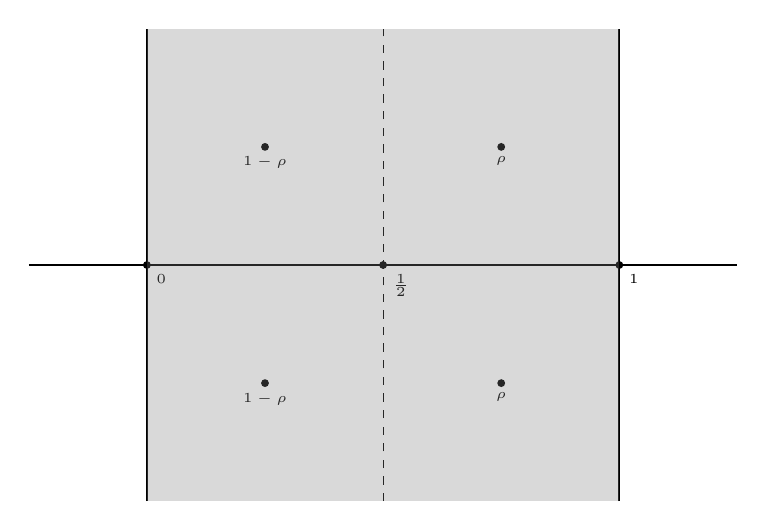
\begin{tikzpicture}[scale=3]
        \def\xmin{-0.5} \def\xmax{2.5}
        \def\ymin{-1} \def\ymax{1}
        \draw[thick] (\xmin,0) -- (\xmax,0);
        \draw[thick] (0,\ymin) -- (0,\ymax);
        \draw[thick] (2,\ymin) -- (2,\ymax);
        \draw[dashed] (1,\ymin) -- (1,\ymax);

        \node at (1.5,0.5) [circle,fill,inner sep=1pt]{};
        \node at (1.5,0.5) [below] {\tiny{\(\rho\)}};
        \node at (0.5,0.5) [circle,fill,inner sep=1pt]{};
        \node at (0.5,0.5) [below] {\tiny{\(1-\conj{\rho}\)}};
        \node at (1.5,-0.5) [circle,fill,inner sep=1pt]{};
        \node at (1.5,-0.5) [below] {\tiny{\(\conj{\rho}\)}};
        \node at (0.5,-0.5) [circle,fill,inner sep=1pt]{};
        \node at (0.5,-0.5) [below] {\tiny{\(1-\rho\)}};

        \node at (0,0) [below right] {\tiny{\(0\)}};
        \node at (0,0) [circle,fill,inner sep=1pt]{};
        \node at (1,0) [below right] {\tiny{\(\frac{1}{2}\)}};
        \node at (1,0) [circle,fill,inner sep=1pt]{};
        \node at (2,0) [below right] {\tiny{\(1\)}};
        \node at (2,0) [circle,fill,inner sep=1pt]{};

        \begin{scope}
          \path[clip] (0,\ymin) -- (0,\ymax) -- (2,\ymax) -- (2,\ymin) -- cycle;
          \fill[gray,opacity=0.3] (0,\ymin) rectangle (2,\ymax);
        \end{scope}
        \end{tikzpicture}
      \caption{Symmetric nontrivial zeros.}
      \label{fig:symmetric_nontrivial_zeros}
    \end{figure}

    The \textit{Riemann hypothesis} for \(L(s)\) says that this symmetry should be as simple as possible:

    \begin{conjecture*}[Riemann hypothesis, \(L(s)\)]
      For the \(L\)-function \(L(s)\), all of the nontrivial zeros lie on the line \(\s = \frac{1}{2}\).
    \end{conjecture*}

    Somewhat confusingly, do not expect the Riemann hypothesis to hold for just any \(L\)-function but we expect it to hold for many \(L\)-functions. In particular, the \textit{grand Riemann hypothesis} says that this symmetry should hold for any \(L\)-function in the Selberg class:

    \begin{conjecture*}[Grand Riemann hypothesis]
      For any Selberg class \(L\)-function \(L(s)\), all of the nontrivial zeros lie on the line \(\s = \frac{1}{2}\).
    \end{conjecture*}

    So far, the Riemann hypothesis remains completely out of reach for any \(L\)-function and thus the grand Riemann hypothesis does as well.
  \section{The Lindel\"of Hypothesis and Convexity Bounds}
    Instead of asking about the zeros of an \(L\)-function \(L(s)\) on the critical line, we can ask about the growth of \(L(s)\), and more generally its derivatives, on the critical line. More precisely, we want to derive an upper bound for \(L(s)\), or one of its derivatives, on the critical line using the Phragm\'en-Lindel\"of convexity principle. The argument we will describe for \(L(s)\) is essentially a refinement of the proof of \cref{prop:L_function_bounded_in_vertical_strips}. Let
    \[
      p_{r_{f}}(s) = \left(\frac{s-1}{s+1}\right)^{r_{f}}.
    \]
    Note that \(p_{r_{f}}(s) \sim 1\). The first step is to guarantee the Phragm\'en-Lindel\"of convexity principle for \(p_{r_{f}}(s)L(s)\) in a region containing the critical strip. As \(L(s)\) is of order \(1\), this is assured (see \cref{append:The_Phragmen_Lindelof_Convexity_principle}). Therefore, we are reduced to estimating the growth of \(p_{r_{f}}(s)L(s)\) for \(\s\) to the left of \(0\) and to the right of \(1\). That is, just outside the edges of the critical strip. The right edge is easily estimated by setting \(\s = 1+\e\) so that
    \[
      p_{r_{f}}(1+\e+it)L(1+\e+it,f) \ll_{\e} 1,
    \]
    which holds since \(L(s)\) is defined by a locally absolutely uniformly convergent Dirichlet series for \(\s > 1\). The left edge is only slightly more difficult. Upon isolating \(L(s)\) in the functional equation, we have
    \[
      L(s) = \e_{L}Q^{\frac{1}{2}-s}\frac{L_{\infty}(1-s)}{L_{\infty}(s)}L(1-s).
    \]
    Applying \cref{equ:gamma_factor_analytic_conductor_estimate} result in the bound
    \[
      L(s) \ll_{\e} \mf{q}(s)^{\frac{1}{2}-\s}L(1-s),
    \]
    for \(s\) in any vertical strip with distance \(\e\) away from the poles of \(L_{\infty}(1-s)\). Multiplying both sides by \(p_{r_{f}}(s)\) and taking \(\s = -\e\), it follows that
    \[
      p_{r_{f}}(-\e+it)L(-\e+it,f) \ll_{\e} \mf{q}(s)^{\frac{1}{2}+\e},
    \]
    which holds since \(L(1-s)\) is defined by a locally absolutely uniformly convergent Dirichlet series for \(\s < 0\). As \(p_{r_{f}}(s)L(s)\) is holomorphic in a region containing the vertical strip \(-\e \le \s \le 1+\e\) and \(p_{r_{f}}(s) \sim 1\), the Phragm\'en-Lindel\"of convexity principle gives
    \begin{equation}\label{equ:convexity_bound_for_L_function_in_critial_strip}
      L(s) \ll_{\e} \mf{q}(s)^{\frac{1-\s}{2}+\e},
    \end{equation}
    in the vertical strip \(-\e \le \s \le 1+\e\) provided \(s\) is distance \(\e\) away from the pole of \(L(s)\) at \(s = 1\) if it exists. At the critical line \cref{equ:convexity_bound_for_L_function_in_critial_strip} gives the following \textit{convexity bound}:
    \[
      L\left(\frac{1}{2}+it,f\right) \ll_{\e} \mf{q}\left(\frac{1}{2}+it,f\right)^{\frac{1}{4}+\e}.
    \]
    The \textit{Lindel\"of hypothesis} for \(L(s)\) says that the exponent can be reduced to \(\e\):

    \begin{conjecture*}[Lindel\"of hypothesis, \(L(s)\)]
      The \(L\)-function \(L(s)\) satisfies
      \[
        L\left(\frac{1}{2}+it,f\right) \ll_{\e} \mf{q}\left(\frac{1}{2}+it,f\right)^{\e}.
      \]
    \end{conjecture*}

    Just as for the Riemann hypothesis, we do not expect the Lindel\"of hypothesis to hold for just any \(L\)-function. Accordingly, the \textit{grand Lindel\"of hypothesis} says that the exponent can be reduced to \(\e\) for any \(L\)-function in the Selberg class and we expect this to hold:

    \begin{conjecture*}[Grand Lindel\"of hypothesis]
      Any Selberg class \(L\)-function \(L(s)\) satisfies
      \[
        L\left(\frac{1}{2}+it,f\right) \ll_{\e} \mf{q}\left(\frac{1}{2}+it,f\right)^{\e}.
      \]
    \end{conjecture*}

    Like the Riemann hypothesis, we have been unable to prove the Lindel\"of hypothesis for any \(L\)-function. However, the Lindel\"of hypothesis seems to be much more tractable. Generally speaking, any improvement upon the exponent in the convexity bound in any aspect of the analytic conductor is called a \textit{subconvexity estimate} (or a \textit{convexity breaking bound}). In other words, we would want a bound of the form
    \[
      L\left(\frac{1}{2}+it,f\right) \ll_{\e} \mf{q}\left(\frac{1}{2}+it,f\right)^{\d+\e},
    \]
    for some \(0 \le \d \le \frac{1}{4}\). The convexity bound says that we may take \(\d = \frac{1}{4}\) while the Lindel\"of hypothesis for \(L(s)\) implies that we may take \(\d = 0\). Subconvexity estimates are viewed with great interest. This is primarily because of their connection to the associated Lindel\"of hypothesis, but also because any improvement upon the convexity bound (or current best value of of \(\d\)) for an \(L\)-function has drastic consequences in applications.

    \begin{remark}
      Some subconvexity bounds are deserving of names. The cases \(\d = \frac{3}{16}\) and \(\d = \frac{1}{6}\) are referred to as the \textit{Burgess bound} and \textit{Weyl bound} respectively.
    \end{remark}
    
    With a little more work, we can obtain a a similar bound for \(L^{(k)}(s)\) for any \(k \ge 1\). First observe that \cref{equ:convexity_bound_for_L_function_in_critial_strip} implies
    \[
      L(s) \ll_{\e} \mf{q}\left(\frac{1}{2}+it,f\right)^{\frac{1}{4}+\e},
    \]
    in the vertical strip \(\left|\s-\frac{1}{2}\right| \le \frac{\e}{2}\). This is just slightly stronger than the convexity bound. Now Cauchy's integral formula gives
    \[
      L^{(k)}\left(\frac{1}{2}+it,f\right) = \frac{k!}{2\pi i}\int_{C}\frac{L(s)}{(s-\frac{1}{2}-it)^{k+1}}\,ds \ll_{\e} \int_{C}|L(s)|ds,
    \]
    where \(C\) is the circle about \(\frac{1}{2}+it\) of radius \(\frac{\e}{2}\). These two estimates, and that the disk bounded by \(C\) is compact, together imply the following \textit{convexity bound}:
    \[
      L^{(k)}\left(\frac{1}{2}+it,f\right) \ll_{\e} \mf{q}\left(\frac{1}{2}+it,f\right)^{\frac{1}{4}+\e}.
    \]
  \section{Estimates on the Critical Line}
    The Lindel\"of hypothesis is concerned with the growth of the \(L\)-function \(L(s)\) along the critical line. Here we provide a way to obtain estimates for \(L(s)\) at \(s = \frac{1}{2}+it\) in terms of finite sums. First, let \(\psi(y)\) be a bump function with compact support in \(\left[\frac{1}{2},2\right]\). For example, we may take
    \[
      \psi(y) = \begin{cases} e^{-\frac{1}{9-(4y-5)^{2}}} & \text{if \(|4y-5| < 3\)}, \\ 0 & \text{if \(|4y-5| \ge 3\)}. \end{cases}
    \]
    Now for an \(L\)-function \(L(s)\), \(t \in \R\), and \(X > 0\), we set
    \[
      A_{\psi}(X,t,f) = \sum_{n \ge 1}a(n)n^{-it}\psi\left(\frac{n}{X}\right),
    \]
    and will suppress the dependence upon \(t\) if \(t = 0\). Our result is the following:

    \begin{theorem}\label{thm:critical_line_estimate}
      Let \(L(s)\) be an \(L\)-function and let \(\psi(y)\) be a bump function with compact support in \(\left[\frac{1}{2},2\right]\). Then
      \[
        L\left(\frac{1}{2}+it,f\right) \ll \max_{X \ll \sqrt{\mf{q}\left(\frac{1}{2}+it,f\right)}}\left(\left|\frac{A_{\psi}(X,t,f)}{\mf{q}\left(\frac{1}{2}+it,f\right)^{\frac{1}{4}}}\right|\right).
      \]
    \end{theorem}
    \begin{proof}
      Taking \(s = \frac{1}{2}+it\), \(X = 1\), and \(\Phi(u) = \cos^{-4d_{f}M}\left(\frac{\pi u}{4M}\right)\) for some integer \(M \ge 1\) in the approximate functional equation gives
      \begin{align*}
        L\left(\frac{1}{2}+it,f\right) &= \sum_{n \ge 1}\frac{a(n)}{n^{\frac{1}{2}+it}}V_{\frac{1}{2}+it}\left(\frac{n}{\sqrt{Q}}\right) \\
        &+ \e\left(\frac{1}{2}+it,f\right)\sum_{n \ge 1}\frac{\conj{a(n)}}{n^{\frac{1}{2}-it}}V_{\frac{1}{2}-it}\left(\frac{n}{\sqrt{Q}}\right)+\frac{R\left(\frac{1}{2}+it,1,f\right)}{Q^{\frac{1}{4}}\g\left(\frac{1}{2}+it,f\right)}.
      \end{align*}
      By \cref{equ:gamma_factor_analytic_conductor_estimate}, we have \(\e\left(\frac{1}{2}+it,f\right) \ll 1\) and therefore we obtain the weaker estimate
      \[
        L\left(\frac{1}{2}+it,f\right) \ll \left|\sum_{n \ge 1}\frac{a(n)n^{-it}}{\sqrt{n}}V_{\frac{1}{2}+it}\left(\frac{n}{\sqrt{Q}}\right)\right|+\left|\sum_{n \ge 1}\frac{\conj{a(n)}n^{it}}{\sqrt{n}}V_{\frac{1}{2}-it}\left(\frac{n}{\sqrt{Q}}\right)\right|+\left|\frac{R\left(\frac{1}{2}+it,f\right)}{Q^{\frac{1}{4}}\g\left(\frac{1}{2}+it,f\right)}\right|.
      \]
      \cref{equ:modified_gamma_estimates,equ:choice_for_V_decay_estimate} together imply that the third term exhibits exponential decay and is therefore absolutely bounded. Hence
      \[
        L\left(\frac{1}{2}+it,f\right) \ll \left|\sum_{n \ge 1}\frac{a(n)n^{-it}}{\sqrt{n}}V_{\frac{1}{2}+it}\left(\frac{n}{\sqrt{Q}}\right)\right|+\left|\sum_{n \ge 1}\frac{\conj{a(n)}n^{it}}{\sqrt{n}}V_{\frac{1}{2}-it}\left(\frac{n}{\sqrt{Q}}\right)\right|.
      \]
      It remains to estimate the two term on the right-hand side. To this end, consider the set of functions \(\left\{\psi\left(\frac{y}{2^{k}}\right)\right\}_{k \in \Z}\). Since \(\psi\left(\frac{y}{2^{k}}\right)\) has support in \([2^{k-1},2^{k+1}]\), the sum \(\s(y) = \sum_{k \in \Z}\psi\left(\frac{y}{2^{k}}\right)\), defined for \(y > 0\), is bounded since at most finitely many terms are nonzero for every \(y\). It is also bounded away from zero since for any \(y > 0\) there is some \(k \in \Z\) for which \(2^{k} \le y \le 3 \cdot 2^{k-1}\) so that \(\frac{y}{2^{k}}\) is at least distance \(\frac{1}{2}\) from the endpoints of \(\left[\frac{1}{2},2\right]\). Together these facts mean that \(\s(y) \asymp 1\). Defining \(\psi_{k}(y) = \psi\left(\frac{y}{2^{k}}\right)\s(y)^{-1}\), it follows that \(\left\{\psi_{k}(y)\right\}_{k \in \Z}\) satisfies
      \[
        \sum_{k \in \Z}\psi_{k}(y) = 1,
      \]
      for any \(y > 0\). Then we can write
      \[
        V_{s}(y) = \sum_{k \in \Z}\psi_{k}(y)V_{s}(y).
      \]
      For the first term, it follows that
      \begin{align*}
        \sum_{n \ge 1}\frac{a(n)n^{-it}}{\sqrt{n}}V_{\frac{1}{2}+it}\left(\frac{n}{\sqrt{Q}}\right) &= \sum_{n \ge 1}\frac{a(n)}{\sqrt{n}}\sum_{k \in \Z}\psi_{k}\left(\frac{n}{\sqrt{Q}}\right)V_{\frac{1}{2}}\left(\frac{n}{\sqrt{Q}}\right) \\
        &= \sum_{k \in \Z}\sum_{n \ge 1}\frac{a(n)n^{-it}}{\sqrt{n}}\psi_{k}\left(\frac{n}{\sqrt{Q}}\right)V_{\frac{1}{2}+it}\left(\frac{n}{\sqrt{Q}}\right) && \text{FTT} \\
        &\ll \sum_{k \in \Z}\left|\sum_{n \ll \sqrt{\mf{q}\left(\frac{1}{2}+it,f\right)}}\frac{a(n)n^{-it}}{\sqrt{n}}\psi_{k}\left(\frac{n}{\sqrt{Q}}\right)\right| \\
        &\ll \sum_{k \ll \log{\mf{q}_{\infty}\left(\frac{1}{2}+it\right)}}\left|\sum_{2^{k-1}\sqrt{Q} \le n \le 2^{k+1}\sqrt{Q}}\frac{a(n)n^{-it}}{\sqrt{n}}\psi_{k}\left(\frac{n}{\sqrt{Q}}\right)\right| \\
        &\ll \max_{X \ll \sqrt{\mf{q}\left(\frac{1}{2}+it,f\right)}}\left(\left|\sum_{\frac{X}{2} \le n \le 2X}\frac{a(n)n^{-it}}{\mf{q}\left(\frac{1}{2}+it,f\right)^{\frac{1}{4}}}\psi\left(\frac{n}{X}\right)\right|\right),
      \end{align*}
      where in the third line we have used that \(V_{\frac{1}{2}+it}\left(\frac{n}{\sqrt{Q}}\right)\) is bounded for \(n \ll \sqrt{\mf{q}\left(\frac{1}{2}+it,f\right)}\) and then exhibits polynomial decay of arbitrarily large order thereafter by \cref{prop:V_function_decay}, in the second to last line we have used that \(\psi_{k}(y)\) has compact support in \([2^{k-1},2^{k+1}]\), and in the last line we have used that \(\s(y) \asymp 1\). In view of the fact that
      \[
        \left|\sum_{n \ge 1}\frac{\conj{a(n)}n^{it}}{\sqrt{n}}V_{\frac{1}{2}-it}\left(\frac{n}{\sqrt{Q}}\right)\right| = \left|\sum_{n \ge 1}\frac{a(n)n^{-it}}{\sqrt{n}}\conj{V_{\frac{1}{2}-it}\left(\frac{n}{\sqrt{Q}}\right)}\right|,
      \]
      the same estimate holds for the second term as well. As
      \[
        \sum_{\frac{X}{2} \le n \le 2X}\frac{a(n)n^{-it}}{\mf{q}\left(\frac{1}{2}+it,f\right)^{\frac{1}{4}}}\psi\left(\frac{n}{X}\right) = \frac{A_{\psi}(2X,t,f)}{\mf{q}\left(\frac{1}{2}+it,f\right)^{\frac{1}{4}}}-\frac{A_{\psi}\left(\frac{X}{2},t,f\right)}{\mf{q}\left(\frac{1}{2}+it,f\right)^{\frac{1}{4}}},
      \]
      we have
      \[
        \max_{X \ll \sqrt{\mf{q}\left(\frac{1}{2}+it,f\right)}}\left(\left|\sum_{\frac{X}{2} \le n \le 2X}\frac{a(n)n^{-it}}{\mf{q}\left(\frac{1}{2}+it,f\right)^{\frac{1}{4}}}\psi\left(\frac{n}{X}\right)\right|\right) \ll \max_{X \ll \sqrt{\mf{q}\left(\frac{1}{2}+it,f\right)}}\left(\left|\frac{A_{\psi}(X,t,f)}{\mf{q}\left(\frac{1}{2}+it,f\right)^{\frac{1}{4}}}\right|\right).
      \]
      Putting everything together, we find that
      \[
       \left|\sum_{n \ge 1}\frac{a(n)n^{-it}}{\sqrt{n}}V_{\frac{1}{2}+it}\left(\frac{n}{\sqrt{Q}}\right)\right|+\left|\sum_{n \ge 1}\frac{\conj{a(n)}n^{it}}{\sqrt{n}}V_{\frac{1}{2}-it}\left(\frac{n}{\sqrt{Q}}\right)\right| \ll \max_{X \ll \sqrt{\mf{q}\left(\frac{1}{2}+it,f\right)}}\left(\left|\frac{A_{\psi}(X,t,f)}{\mf{q}\left(\frac{1}{2}+it,f\right)^{\frac{1}{4}}}\right|\right),
      \]
      completing the proof.
    \end{proof}

    In view of \cref{thm:central_value_estimate}, it suffices to bound \(A_{\psi}(X,t,f)\) for \(X \ll \sqrt{\mf{q}\left(\frac{1}{2}+it,f\right)}\) to estimate \(L\left(\frac{1}{2}+it,f\right)\). Moreover, we obtain the convexity bound from \cref{thm:central_value_estimate} by using that \(a(n) \ll_{\e} n^{\e}\) to obtain the estimate
    \begin{equation}\label{equ:coefficient_sum_trivial_bound}
      \max_{X \ll \sqrt{\mf{q}\left(\frac{1}{2}+it,f\right)}}|A_{\psi}(X,t,f)| \ll_{\e} \int_{\frac{1}{2}\sqrt{\mf{q}\left(\frac{1}{2}+it,f\right)}}^{2\sqrt{\mf{q}\left(\frac{1}{2}+it,f\right)}}x^{\e}\,dx \ll_{\e} \mf{q}\left(\frac{1}{2}+it,f\right)^{\frac{1}{2}+\e}.
    \end{equation}
    
    \begin{remark}
      Recall that we expect \(L(s)\) to satisfy the Lindel\"of hypothesis if \(L(s)\) is of Selberg class. This means, in the Selberg class case, that we should expect lots of cancellation in the sum \(A_{\psi}(X,t,f)\). In fact, the expected cancellation should be \(O\left(\mf{q}\left(\frac{1}{2}+it,f\right)^{\frac{1}{4}}\right)\) from that in \cref{equ:coefficient_sum_trivial_bound}. As the coefficients \(a(n)\) may very well be real, much of this cancellation should come from the terms \(n^{-it} = e^{-it\log(n)}\) which acts on \(a(n)\) by rotation (since \(|n^{-it}| = 1\)).
    \end{remark}

    Sometimes, however, we are only concerned with the size of \(L(s)\) at the central point. The value of \(L(s)\) at the central point is called the \textit{central value} of \(L(s)\). Many important properties about \(L(s)\) can be connected to its central value. Any argument used to estimate the central value of an \(L\)-function is called a \textit{central value estimate}. Taking \(t = 0\) in \cref{thm:critical_line_estimate} gives a way to obtain central value estimates:

    \begin{theorem}\label{thm:central_value_estimate}
      Let \(L(s)\) be an \(L\)-function and let \(\psi(y)\) be a bump function with compact support in \(\left[\frac{1}{2},2\right]\). Then
      \[
        L\left(\frac{1}{2},f\right) \ll \max_{X \ll \sqrt{Q}}\left(\left|\frac{A_{\psi}(X,f)}{Q^{\frac{1}{4}}}\right|\right).
      \]
    \end{theorem}
    \begin{proof}
      Take \(t = 0\) in \cref{thm:critical_line_estimate} and recall that \(\mf{q}\left(\frac{1}{2},f\right) \asymp Q\).
    \end{proof}

    Indeed, \cref{thm:central_value_estimate} shows that it suffices to bound \(A_{\psi}(X,f)\) for \(X \ll \sqrt{Q}\) to estimate the central value of \(L(s)\).
  \section{Logarithmic Derivatives}
    There is an incredibly useful formula for the logarithmic derivative of any \(L\)-function which is often the starting point for deeper analytic investigations. To deduce it, we will need a more complete understanding of \(\L(s)\). First observe that the zeros \(\rho\) of \(\L(s)\) are contained inside of the critical strip. Indeed, we have already remarked that \(L(s)\) has no zeros for \(\s > 0\) and clearly \(L_{\infty}(s)\) does not have zeros in this region as well. Therefore \(\L(s)\) is nonzero for \(\s > 1\). By the functional equation, \(\L(s)\) is also nonzero for \(\s < 0\) too. In other words, the zeros of \(\L(s)\) are the nontrivial zeros of \(L(s)\). Before we state our result, we setup some notation. For an \(L\)-function \(L(s)\) we define
    \[
      \xi(s) = (s(1-s))^{r_{f}}\L(s).
    \]
    Note that \(\xi(s)\) is essentially just \(\L(s)\) with the potential poles at \(s = 0\) and \(s = 1\) removed. From the functional equation, we also have
    \[
      \xi(s) = \e_{L}\xi(1-s,\conj{f}).
    \]
    We now state our desired result:

    \begin{proposition}\label{prop:explicit_formula_log_derivative}
      For any \(L\)-function \(L(s)\), there exist constants \(A(f)\) and \(B(f)\) such that
      \[
        \xi(s) = e^{A(f)+B(f)s}\prod_{\rho \neq 0,1}\left(1-\frac{s}{\rho}\right)e^{\frac{s}{\rho}},
      \]
      and hence the sum
      \[
        \sum_{\rho \neq 0,1}\frac{1}{|\rho|^{1+\e}},
      \]
      is convergent provided the product and sum are both counted with multiplicity and ordered with respect to the size of the ordinate. Moreover,
      \[
        -\frac{L'}{L}(s) = \frac{r_{f}}{s}+\frac{r_{f}}{s-1}+\frac{1}{2}\log{Q}+\frac{\g'}{\g}(s)-B(f)-\sum_{\rho \neq 0,1}\left(\frac{1}{s-\rho}+\frac{1}{\rho}\right).
      \] 
    \end{proposition}
    \begin{proof}
      For the first statement, observe that \(\xi(s)\) is entire since the only possible poles of \(\L(s)\) are at \(s = 0\) and \(s = 1\) and are of order \(r_{f}\). We also claim that \(\xi(s)\) is of order \(1\). By the functional equation, it suffices to show this for \(\s \ge \frac{1}{2}\). This follows from \(L(s)\) being of order \(1\) and \cref{equ:modified_gamma_estimates} (within \(\e\) of the poles of \(L_{\infty}(s)\) we know \(\xi(s)\) is bounded because it is entire). By the Hadamard factorization theorem (see \cref{append:Factorizations_and_Finite_Order}),
       \[
        \xi(s) = e^{A(f)+B(f)s}\prod_{\rho \neq 0,1}\left(1-\frac{s}{\rho}\right)e^{\frac{s}{\rho}},
      \]
      for some constants \(A(f)\) and \(B(f)\) and the desired sum converges. This proves the first statement. For the second, taking the logarithmic derivative of the definition of \(\xi(s)\) yields
      \begin{equation}\label{equ:log_derivative_1}
        \frac{\xi'}{\xi}(s) = \frac{r_{f}}{s}+\frac{r_{f}}{s-1}+\frac{1}{2}\log{Q}+\frac{\g'}{\g}(s)+\frac{L'}{L}(s).
      \end{equation}
      On the other hand, taking the logarithmic derivative of the Hadamard factorization gives
      \begin{equation}\label{equ:log_derivative_2}
        \frac{\xi'}{\xi}(s) = B(f)+\sum_{\rho \neq 0,1}\left(\frac{1}{s-\rho}+\frac{1}{\rho}\right).
      \end{equation}
      Equating \cref{equ:log_derivative_1,equ:log_derivative_2}, we arrive at
      \[
        B(f)+\sum_{\rho \neq 0,1}\left(\frac{1}{s-\rho}+\frac{1}{\rho}\right) = \frac{r_{f}}{s}+\frac{r_{f}}{s-1}+\frac{1}{2}\log{Q}+\frac{\g'}{\g}(s)+\frac{L'}{L}(s).
      \]
      Isolating \(-\frac{L'}{L}(s)\) completes the proof.
    \end{proof}

    We now need to make a few comments. Our first is regarding the constants \(A(f)\) and \(B(f)\). The explicit evaluation of these constants can be challenging and heavily depends upon the arithmetic object \(f\). However, useful estimates are not too difficult to obtain. We also claim \(A(\conj{f}) = \conj{A(f)}\) and \(B(\conj{f}) = \conj{B(f)}\). To see this, recall that \(L(\conj{s},\conj{f}) = \conj{L(s)}\). Then \(\xi(\conj{s},\conj{f}) = \conj{\xi(s)}\) because \(\g(s,\conj{f}) = L_{\infty}(s)\), the \(\k_{j}\) are real or occur in conjugate pairs, and \(\G(\conj{s}) = \conj{\G(s)}\). But then the functional equation and \cref{prop:explicit_formula_log_derivative} together imply
    \[
      e^{A(\conj{f})+B(\conj{f})s} = \frac{\xi'}{\xi}(0,\conj{f}) = \conj{\frac{\xi'}{\xi}(0,f)} = e^{\conj{A(f)}+\conj{B(f)}s},
    \]
    and the claim follows. Our second comment concerns the negative logarithmic derivative of \(L(s)\). In general, this function attracts much attention for analytic investigations. As \(L(s)\) is holomorphic for \(\s > 1\) and admits an Euler product there, we can take the logarithm of the Euler product (turning it into a sum) and differentiate termwise to obtain
    \begin{equation}\label{equ:log_derivaive_direct_computation}
      -\frac{L'}{L}(s) = -\sum_{p}\sum_{j}\frac{d}{ds}\log(1-\a_{j}(p)p^{-s}) = \sum_{p}\sum_{j}\frac{\a_{j}(p)\log(p)}{(1-\a_{j}(p)p^{-s})p^{s}}.
    \end{equation}
    From the Taylor series of \(\frac{1}{1-s}\), it follows that \(-\frac{L'}{L}(s)\) is a locally absolutely uniformly convergent Dirichlet series of the form
    \[
       -\frac{L'}{L}(s) = \sum_{n \ge 1}\frac{\L_{L}(n)}{n^{s}},
    \]
    for \(\s > 1\), where
    \[
      \L_{L}(n) = \begin{cases} \sum_{j}\a_{j}(p)^{k}\log(p) & \text{if \(n = p^{k}\) for some \(k \ge 1\)}, \\ 0 & \text{otherwise}. \end{cases}
    \]
    It is worth noting that \(\L_{\conj{f}}(n) = \conj{\L_{L}(n)}\).
  \section{Zero Density}
    The deepest subject of the theory of \(L\)-functions is arguably the distribution of the zeros of \(L\)-functions. Here we introduce a method of counting zeros of \(L\)-functions and gaining a very simple understanding of their density as a result. We first require an immensely useful lemma:

    \begin{lemma}\label{lem:powerful_L-function_approximation_lemma}
      Let \(L(s)\) be an \(L\)-function. The following statements hold:
      \begin{enumerate}[label*=(\roman*)]
        \item The constant \(B(f)\) satisfies
        \[
          \Re(B(f)) = -\sum_{\rho \neq 0,1}\Re\left(\frac{1}{\rho}\right),
        \]
        where the sum is counted with multiplicity and ordered with respect to the size of the ordinate.
        \item For any \(T \ge 0\), the number of nontrivial zeros \(\rho = \b+i\g\) with \(\rho \neq 0,1\) and such that \(|T-\g| \le 1\) is \(O(\log{\mf{q}(iT,f)})\).
        \item For \(\s > 1\), we have
        \[
          \Re\left(\frac{1}{s-\rho}\right) > 0 \quad \text{and} \quad \Re\left(\frac{1}{s+\k_{j}}\right) > 0.
        \]
        \item We have
        \[
          -\frac{L'}{L}(s) = \frac{r_{f}}{s}+\frac{r_{f}}{s-1}-\sum_{|s+\k_{j}| < 1}\frac{1}{s+\k_{j}}-\sum_{\substack{|s-\rho| < 1 \\ \rho \neq 0,1}}\frac{1}{s-\rho}+O(\log{\mf{q}(s)}),
        \]
        for any \(s\) in the vertical strip \(-\frac{1}{2} \le \s \le 2\). Moreover, in this vertical strip we also have
        \[
          \Re\left(-\frac{L'}{L}(s)\right) \le \Re\left(\frac{r_{f}}{s}\right)+\Re\left(\frac{r_{f}}{s-1}\right)-\sum_{|s+\k_{j}| < 1}\Re\left(\frac{1}{s+\k_{j}}\right)-\sum_{\substack{|s-\rho| < 1 \\ \rho \neq 0,1}}\Re\left(\frac{1}{s-\rho}\right)+O(\log{\mf{q}(s)}),
        \]
        and we may discard any term in either sum if \(1 < \s \le 2\).
      \end{enumerate}
    \end{lemma}
    \begin{proof}
      We will prove each statement separately.
      \begin{enumerate}[label*=(\roman*)]
        \item To prove (i), first recall that  \(B(\conj{f}) = \conj{B(f)}\). Then \cref{equ:log_derivative_2} and the functional equation together imply
        \[
          2\Re(B(f)) = B(f)+B(\conj{f}) = -\sum_{\rho \neq 0,1}\left(\frac{1}{s-\rho}+\frac{1}{1-s-\conj{\rho}}+\frac{1}{\rho}+\frac{1}{\conj{\rho}}\right),
        \]
        where we have made use of the fact that the nontrivial zeros occur is pairs \(\rho\) and \(1-\conj{\rho}\) where the latter is also a nontrivial zero of \(L(1-s,\conj{f})\). Now fix \(s\) such that it does not coincide with the ordinate of a nontrivial zero. Then \(s\) is bounded away from all of the nontrivial zeros and it follows that \(\frac{1}{(s-\rho)}+\frac{1}{(1-s-\conj{\rho})} \ll \frac{1}{\rho^{2}}\) and \(\frac{1}{\rho}+\frac{1}{\conj{\rho}} \ll \frac{1}{\rho^{2}}\). Therefore the sums
        \[
          \sum_{\rho \neq 0,1}\left(\frac{1}{s-\rho}+\frac{1}{1-s-\conj{\rho}}\right) \quad \text{and} \quad \sum_{\rho \neq 0,1}\left(\frac{1}{\rho}+\frac{1}{\conj{\rho}}\right),
        \]
        converge absolutely by \cref{prop:explicit_formula_log_derivative} and so we can sum them separately. The first sum vanishes by again using the fact that the nontrivial zeros occur is pairs \(\rho\) and \(1-\conj{\rho}\). Thus
        \[
          2\Re(B(f)) = \sum_{\rho \neq 0,1}\left(\frac{1}{\rho}+\frac{1}{\conj{\rho}}\right) = -\sum_{\rho \neq 0,1}\Re\left(\frac{1}{\rho}\right),
        \]
        which gives (i).
        \item For (ii), we first bound two important quantities. For the first quantity, the definition of \(\L_{L}(n)\) and that \(|\a_{j}(p)| \le p\) together imply the weak bound \(|\L_{L}(n)| \le d_{f}n\log(n)\). Then
        \begin{equation}\label{equ:log_derivative_bound_conductor}
          \frac{L'}{L}(s) \ll d_{f}\z'(s-1) \ll \log{\mf{q}(f)},
        \end{equation}
        provided \(\s > 2\). For the second quantity, \cref{equ:digamma_gamma_factor_analytic_conductor_estimate} implies
        \begin{equation}\label{equ:log_conductor_gamma_factor_bound_analytic_conductor}
          \frac{1}{2}\log{Q}+\frac{\g'}{\g}(s) \ll \log{\mf{q}(s)},
        \end{equation}
        for \(\s > 0\). Now fix \(T \ge 0\) and let \(s = 3+iT\). Taking the real part of the formula for the negative logarithmic derivative in \cref{prop:explicit_formula_log_derivative} and combining \cref{equ:log_derivative_bound_conductor,equ:log_conductor_gamma_factor_bound_analytic_conductor} with (i) results in
        \[
          \sum_{\rho \neq 0,1}\Re\left(\frac{1}{s-\rho}\right) \ll \log{\mf{q}(iT,f)}.
        \]
        But as
        \[
          \frac{2}{9+(T-\g)^{2}} \le \Re\left(\frac{1}{s-\rho}\right) \le \frac{3}{4+(T-\g)^{2}},
        \]
        we obtain
        \begin{equation}\label{equ_sum_of_nontrivial_zeros_log_analytic_conductor_bound}
          \sum_{\rho \neq 0,1}\frac{1}{1+(T-\g)^{2}} \ll \log{\mf{q}(iT,f)},
        \end{equation}
        which is stronger than the first statement of (ii) since all of the terms in the sum are positive. The second statement is also clear.
        \item For (iii), just observe that
        \[
          \Re\left(\frac{1}{s-\rho}\right) = \frac{\s-\b}{(\s-\b)^{2}+(t-
          g)^{2}} > 0 \quad \text{and} \quad \Re\left(\frac{1}{s+\k_{j}}\right) = \frac{\s+\Re(\k_{j})}{(\s+\Re(\k_{j}))^{2}+(t+\Im(\k_{j}))^{2}} > 0,
        \]
        where the first bound holds because \(\b \le 1\) and the second bound holds because \(\Re(\k_{j}) > -1\).
        \item To deduce (iv), let \(s\) be such that \(-\frac{1}{2} \le \s \le 2\). Using \cref{equ:log_derivative_bound_conductor}, we can write
        \[
          -\frac{L'}{L}(s) = -\frac{L'}{L}(s)+\frac{L'}{L}(3+it,f)+O(\log{\mf{q}(s)}).
        \]
        Applying the formula for the negative logarithmic derivative in \cref{prop:explicit_formula_log_derivative} to the two terms on the right-hand side and using \cref{equ:digamma_gamma_factor_analytic_conductor_estimate} for \(\s > 0\), we get
        \[
          -\frac{L'}{L}(s) = \frac{r_{f}}{s}+\frac{r_{f}}{s-1}+\frac{\g'}{\g}(s)-\sum_{\rho \neq 0,1}\left(\frac{1}{s-\rho}-\frac{1}{3+it-\rho}\right)+O(\log{\mf{q}(s)}).
        \]
        We now estimate the remaining sum. Retain the first part of the terms for which \(|s-\rho| < 1\). The contribution from the second part of these terms is \(O(\log{\mf{q}(it,f)})\) by (ii). For those terms with \(|s-\rho| \ge 1\), we have
        \[
          \left|\frac{1}{s-\rho}-\frac{1}{3+it-\rho}\right| \le \frac{3-\s}{(3-\b)^{2}+(t-\g)^{2}} \le \frac{3}{1+(t-\g)^{2}}.
        \]
        Therefore from \cref{equ_sum_of_nontrivial_zeros_log_analytic_conductor_bound}, the contribution of these terms is \(O(\log{\mf{q}(it,f)})\) too. It follows that
        \[
          -\frac{L'}{L}(s) = \frac{r_{f}}{s}+\frac{r_{f}}{s-1}+\frac{\g'}{\g}(s)-\sum_{\substack{|s-\rho| < 1 \\ \rho \neq 0,1}}\frac{1}{s-\rho}+O(\log{\mf{q}(s)}).
        \]
        Applying \(\frac{\G'}{\G}(s+1) = \frac{\G'}{\G}(s)+\frac{1}{s}\) to \(\frac{\g'}{\g}(s)\) and using \cref{equ:digamma_gamma_factor_analytic_conductor_estimate} gives
        \[
          \frac{\g'}{\g}(s) = -\sum_{|s+\k_{j}| < 1}\frac{1}{s+\k_{j}}+O(\log{\mf{q}_{\infty}(s)}).
        \]
        Then we obtain
        \[
          -\frac{L'}{L}(s) = \frac{r_{f}}{s}+\frac{r_{f}}{s-1}-\sum_{|s+\k_{j}| < 1}\frac{1}{s+\k_{j}}-\sum_{\substack{|s-\rho| < 1 \\ \rho \neq 0,1}}\frac{1}{s-\rho}+O(\log{\mf{q}(s)}),
        \]
        which is the first statement of (iv). For second statement, tak the real part of this estimate and write it as
        \[
          \sum_{|s+\k_{j}| < 1}\Re\left(\frac{1}{s+\k_{j}}\right)+\sum_{\substack{|s-\rho| < 1 \\ \rho \neq 0,1}}\Re\left(\frac{1}{s-\rho}\right) \le \Re\left(-\frac{L'}{L}(s)\right)+\Re\left(\frac{r_{f}}{s}\right)+\Re\left(\frac{r_{f}}{s-1}\right)+O(\log{\mf{q}(s)}).
        \]
        Now observe that we can discard any of the terms in either sum provided \(1 < \s \le 2\) by (iii).
      \end{enumerate}
    \end{proof}

    With \cref{lem:powerful_L-function_approximation_lemma} in hand, we can deduce a result which estimates the number of nontrivial zeros in a box. Accordingly, for any \(T \ge 0\) we define
    \[
      N(T,f) = |\{\rho = \b+i\g \in \C:L(\rho,f) = 0 \text{ with } 0 \le \b \le 1 \text{ and } |\g| \le T\}|.
    \]
    In other words, \(N(T,f)\) is the number of nontrivial zeros of \(L(s)\) with ordinate in \([-T,T]\). We will prove the following asymptotic formula for \(N(T,f)\):

    \begin{theorem}\label{thm:zero_counting}
      For any \(L\)-function \(L(s)\) and \(T \ge 1\),
      \[
        N(T,f) = \frac{T}{\pi}\log\left(\frac{QT^{d_{f}}}{(2\pi e)^{d_{f}}}\right)+O(\log{\mf{q}(iT,f)}).
      \]
      In particular,
      \[
        \frac{N(T,f)}{T} \sim \frac{1}{\pi}\log\left(\frac{QT^{d_{f}}}{(2\pi e)^{d_{f}}}\right).
      \]
    \end{theorem}
    \begin{proof}
      Let \(T \ge 1\) and set
      \[
        N'(T,f) = \left|\{\rho = \b+i\g \in \C:L(\rho,f) = 0 \text{ with } 0 \le \b \le 1 \text{ and } 0 < \g \le T\}\right|.
      \]
      As the nontrivial zeros occur in pairs \(\rho\) and \(1-\conj{\rho}\) where the latter is also a nontrivial zero of \(L(s,\conj{f})\), it follows that
      \[
        N(T,f) = N'(T,f)+N'(T,\conj{f})+O(\log{\mf{q}(f)}),
      \]
      where \(O(\log{\mf{q}(f)})\) accounts for the possible real nontrivial zeros. There are finitely many such nontrivial zeros because the interval \(0 \le s \le 1\) is compact. We will estimate \(N'(T,f)\) and in doing so we may assume \(L(s)\) does not vanish on the line \(t = T\) by varying \(T\) by a sufficiently small constant, if necessary, and observing that \(N(T,f)\) is modified by a quantity of size \(O(\log{\mf{q}(iT,f)})\) by \cref{lem:powerful_L-function_approximation_lemma} (i). Since the nontrivial zeros are isolated, let \(\d > 0\) be small enough such that \(\L(s)\) has no nontrivial zeros for \(-\d \le t < 0\). Then by our previous comments and the argument principle,
      \[
        N'(T,f) = \frac{1}{2\pi i}\int_{\eta}\frac{\xi'}{\xi}(s)\,ds+O(\log{\mf{q}(iT,f)}),
      \]

      \begin{figure}[ht]
        \centering
        \begin{tikzpicture}[scale=3]
          \def\xmin{-1.5} \def\xmax{2.5}
          \def\ymin{-0.5} \def\ymax{2}
          \draw[thick] (\xmin,0) -- (\xmax,0);
          \draw[thick] (0,\ymin) -- (0,\ymax);
          \draw[thick] (1,\ymin) -- (1,\ymax);
          \draw[dashed] (0.5,\ymin) -- (0.5,\ymax);

          \draw[->-] (0.5,-0.1) -- (2,-0.1);
          \draw[->-] (2,-0.1) -- (2,1.5);
          \draw[->-] (2,1.5) -- (0.5,1.5);
          \draw[->-] (0.5,1.5) -- (-1,1.5);
          \draw[->-] (-1,1.5) -- (-1,-0.1);
          \draw[->-] (-1,-0.1) -- (0.5,-0.1);

          \node at (1.25,-0.1) [below] {\tiny{\(\eta_{1}\)}};
          \node at (2,0.7) [right] {\tiny{\(\eta_{2}\)}};
          \node at (1.25,1.5) [above] {\tiny{\(\eta_{3}\)}};
          \node at (-0.25,1.5) [above] {\tiny{\(\eta_{4}\)}};
          \node at (-1,0.7) [left] {\tiny{\(\eta_{5}\)}};
          \node at (-0.25,-0.1) [below] {\tiny{\(\eta_{6}\)}};

          \node at (2,-0.1) [circle,fill,inner sep=1pt]{};
          \node at (2,1.5) [circle,fill,inner sep=1pt]{};
          \node at (0.5,1.5) [circle,fill,inner sep=1pt]{};
          \node at (-1,1.5) [circle,fill,inner sep=1pt]{};
          \node at (-1,-0.1) [circle,fill,inner sep=1pt]{};
          \node at (0.5,-0.1) [circle,fill,inner sep=1pt]{};

          \node at (2,-0.1) [below] {\tiny{\(3-i\d\)}};
          \node at (2,1.5) [above] {\tiny{\(3+iT\)}};
          \node at (0.5,1.5) [above right] {\tiny{\(\frac{1}{2}+iT\)}};
          \node at (-1,1.5) [above] {\tiny{\(-2+iT\)}};
          \node at (-1,-0.1) [below] {\tiny{\(-2-i\d\)}};
          \node at (0.5,-0.1) [below right] {\tiny{\(\frac{1}{2}-i\d\)}};
        \end{tikzpicture}
        \caption{A zero counting contour.}
        \label{fig:zero_counting_contour}
      \end{figure}

      where \(\eta = \sum_{1 \le i \le 6}\eta_{i}\) is the contour in \cref{fig:zero_counting_contour}. Since \(\log(s) = \log{|s|}+i\arg(s)\), we have
      \[
        \frac{1}{2\pi i}\int_{\eta}\frac{\xi'}{\xi}(s)\,ds = \frac{1}{2\pi i}\int_{\eta}\frac{d}{ds}\log{|\xi(s)|}\,ds+\frac{1}{2\pi }\int_{\eta}\frac{d}{ds}\arg\xi(s)\,ds = \frac{1}{2\pi}\D_{\eta}\arg(\xi(s)),
      \]
      where the last equality holds by noting that \(\eta\) is closed so that the first integral vanishes. For convenience, set \(\eta_{L} = \eta_{1}+\eta_{2}+\eta_{3}\) and \(\eta_{R} = \eta_{4}+\eta_{5}+\eta_{6}\). Recall that we have already shown \(\xi(\conj{s},\conj{f}) = \conj{(\xi(s))}\). Using this fact along with the functional equation and that \(-\arg(s) = \arg(\conj{s})\), we compute
      \begin{align*}
        \D_{\eta_{L}}\arg(\xi(s)) &= \D_{\eta_{L}}\arg\left(\e_{L}\xi(1-s,\conj{f})\right) \\
        &= -\D_{\conj{\eta_{R}}}\arg\left(\e_{L}\xi(s,\conj{f})\right) \\
        &= \D_{\conj{\eta_{R}}}\arg\left(\conj{\e_{L}}\xi(\conj{s},f)\right) \\
        &= \D_{\eta_{R}}\arg\left(\conj{\e_{L}}\xi(s)\right) \\
        &= \D_{\eta_{R}}\arg\left(\conj{\e_{L}}\right)+\D_{\eta_{R}}\arg(\xi(s)) \\
        &= \D_{\eta_{R}}\arg(\xi(s)).
      \end{align*}
      In other words, the change in argument along \(\eta_{L}\) is equal to the change in argument along \(\eta_{R}\) and so
      \[
        \frac{1}{2\pi i}\int_{\eta}\frac{\xi'}{\xi}(s)\,ds = \frac{1}{\pi}\D_{\eta_{L}}\arg\xi(s).
      \]
      Thus to estimate the integral, we estimate the change in argument along \(\eta_{L}\) of each factor in
      \[
        \xi(s) = (s(1-s))^{r_{f}}Q^{\frac{s}{2}}\pi^{-\frac{d_{f}s}{2}}\prod_{j}\G\left(\frac{s+\k_{j}}{2}\right)L(s).
      \]
      For the factor \((s(1-s))^{r_{f}}\), we first have
      \[
        \D_{\eta_{L}}\arg(s) = \arg\left(\frac{1}{2}+iT\right)-\arg\left(\frac{1}{2}-i\d\right) = O\left(\frac{1}{T}\right),
      \]
      and
      \[
        \D_{\eta_{L}}\arg(1-s) = \arg\left(\frac{1}{2}-iT\right)-\arg\left(\frac{1}{2}+i\d\right) = O\left(\frac{1}{T}\right),
      \]
      where in both computations we have used \(\arg(s) = \tan^{-1}\left(\frac{t}{\s}\right) = \frac{\pi}{2}+O\left(\frac{1}{t}\right)\), provided \(\s > 0\), which holds by truncating the Laurent series of the inverse tangent after the first term. Combining these two bounds, we obtain
      \begin{equation}\label{equ:zero_counting_1}
        \D_{\eta_{L}}(s(1-s))^{r_{f}} = O\left(\frac{1}{T}\right).
      \end{equation}
      For the factor \(Q^{\frac{s}{2}}\), we use that \(\arg(s) = \Im(\log(s))\) and compute
      \begin{equation}\label{equ:zero_counting_2}
        \D_{\eta_{L}}\arg{Q^{\frac{s}{2}}} = \log{Q}\left(\frac{T}{2}+\frac{\d}{2}\right) = \frac{T}{2}\log{Q}+O(1).
      \end{equation}
      For the factor \(\pi^{-\frac{d_{f}s}{2}}\), we use that \(\arg(s) = \Im(\log(s))\) and compute
      \begin{equation}\label{equ:zero_counting_3}
        \D_{\eta_{L}}\arg\left(\pi^{-\frac{d_{f}s}{2}}\right) = \log\left(\frac{1}{\pi^{d_{f}}}\right)\left(\frac{T}{2}+\frac{\d}{2}\right) = \frac{T}{2}\log\left(\frac{1}{\pi^{d_{f}}}\right)+O(1).
      \end{equation}
      For the factor \(\prod_{j}\G\left(\frac{s+\k_{j}}{2}\right)\), we first use \cref{equ:log_gamma_estimate} (valid since \(T \ge 1\)) and that \(\arg(s) = \Im(\log(s))\) to obtain
      \begin{align*}
        \D_{\eta_{L}}\arg\G(s) &= T\log\left|\frac{1}{2}+iT\right|-T+\d\log\left|\frac{1}{2}+i\d\right|-\d+O(1) \\
        &= T\log(T)-T+O(1) \\
        &= T\log\left(\frac{T}{e}\right)+O(1).
      \end{align*}
      It follows that
      \begin{equation}\label{equ:zero_counting_4}
        \D_{\eta_{L}}\arg\left(\prod_{j}\G\left(\frac{s+\k_{j}}{2}\right)\right) = \frac{T}{2}\log\left(\frac{T^{d_{f}}}{(2e)^{d_{f}}}\right)+O(\log{\mf{q}(f)}).
      \end{equation}
      For the factor \(L(s)\), we again use \(\arg(s) = \Im(\log(s))\) to make the observation that
      \[
        \D_{\eta_{L}}\arg(L(s)) = \Im\left(\int_{\eta_{L}}\frac{L'}{L}(s)\,ds\right).
      \]
      By \cref{equ:log_derivative_bound_conductor}, the integral is \(O(\log{Q})\) on \(\eta_{2}\). On \(\eta_{1}\) and \(\eta_{3}\), \cref{lem:powerful_L-function_approximation_lemma} (ii) and (iv) together imply that the integral is \(O(\log{\mf{q}(iT,f)})\). It follows that
      \begin{equation}\label{equ:zero_counting_5}
        \D_{\eta_{L}}\arg(L(s)) = O(\log{\mf{q}(iT,f)}).
      \end{equation}
      Combining \cref{equ:zero_counting_1,equ:zero_counting_2,equ:zero_counting_3,equ:zero_counting_4,equ:zero_counting_5} results in
      \[
        \frac{1}{\pi}\D_{\eta_{L}}\arg\xi(s) = \frac{T}{2\pi}\log\left(\frac{T^{d_{f}}}{(2\pi e)^{d_{f}}}\right)+O(\log{\mf{q}(iT,f)}),
      \]
      and therefore
      \[
        N'(T,f) = \frac{T}{2\pi}\log\left(\frac{T^{d_{f}}}{(2\pi e)^{d_{f}}}\right)+O(\log{\mf{q}(iT,f)}),
      \]
      The asymptotic formula follows from this estimate and that the same exact estimate holds for \(N'(T,\conj{f})\) by using the \(L\)-function \(L(s,\conj{f})\). We obtain the asymptotic equality at once from the asymptotic formula.
    \end{proof}

    It is worth noting that the main term in the proof of \cref{thm:zero_counting} comes from the change in argument of \(Q^{\frac{s}{2}}L_{\infty}(s)\) along \(\eta_{3}\) (equivalently \(\eta_{4}\)). Moreover, the contribution from \(L(s)\) is only to the error term. This is a good example of how analytic information of an \(L\)-function is intrinsically connected to its gamma factor. Also, with \cref{thm:zero_counting} we can derive our zero density estimate. The asymptotic equivalence in \cref{thm:zero_counting} can be interpreted as saying that for large \(T\) the density of \(N(T,f)\) is approximately \(\frac{1}{\pi}\log\left(\frac{QT^{d_{f}}}{(2\pi e)^{d_{f}}}\right)\). Since this grows as \(T \to \infty\), we see that the nontrivial zeros tend to accumulate farther up the critical strip with logarithmic growth. We can dispense with this accumulation. If \(\rho = \b+i\g\) is a nontrivial zero of \(L(s)\) then we call \(\rho_{\text{unf}} = \b+i\w\) the \textit{unfolded nontrivial zero} corresponding to \(\rho\) where
    \[
      \w = \frac{\g}{\pi}\log\left(\frac{Q|\g|^{d_{f}}}{(2\pi e)^{d_{f}}}\right).
    \]
    Now for any \(W \ge 0\), define
    \[
      N_{\text{unf}}(W,f) = |\{\rho_{\text{unf}} = \b+i\w \in \C:L(\rho,f) = 0 \text{ with } 0 \le \b \le 1 \text{ and } |\w| \le W\}|.
    \]
    In other words, \(N_{\text{unf}}(T,f)\) is the number of unfolded nontrivial zeros of \(L(s)\) with ordinate in \([-W,W]\). We then have the following well-known result:

    \begin{proposition}\label{prop:unfolded_zeros_are_evenly_spaced}
    For any \(L\)-function \(L(s)\) and \(W \ge \frac{1}{\pi}\log\left(\frac{Q}{(2\pi e)^{d_{f}}}\right)\),
    \[
      \frac{N_{\text{unf}}(W,f)}{W} \sim 1.
    \]
    \end{proposition}
    \begin{proof}
      Consider the function \(f(t)\) defined by
      \[
        f(t) = \frac{t}{\pi}\log\left(\frac{Q|t|^{d_{f}}}{(2\pi e)^{d_{f}}}\right),
      \]
      for real \(t\). Since \(f(t)\) is a strictly increasing continuous function, it has an inverse \(g(w)\) for real \(w\). It follows that \(|\w| \le W\) if and only if \(|\rho| \le g(W)\) and so \(N_{\text{unf}}(W,f) = N(g(W),f)\). But by \cref{thm:zero_counting} and that \(g(w)\) is the inverse of \(f(t)\), we have \(N(g(W),f) \sim W\). Then
      \[
        N_{\text{unf}}(W,f) \sim W,
      \]
      which is equivalent to the claim.
    \end{proof}

    We interpret \cref{prop:unfolded_zeros_are_evenly_spaced} as saying that the unfolded nontrivial zeros are evenly spaced opposed to \cref{thm:zero_counting} which say that they tend to accumulate up the critical strip.
  \section{A Zero-free Region}
    Although the Riemann hypothesis remains out of reach, some progress has been made to understand regions inside of the critical strip for which \(L\)-functions are nonzero except for possibly one real exception. Such regions are known as \textit{zero-free regions} and there is great interest in improving the breadth of such regions. We will derive a standard zero-free region for any \(L\)-function under some mild assumptions. First a useful lemma:

    \begin{lemma}\label{lem:non-vanshing_at_1_lemma}
      Let \(L(s)\) be an \(L\)-function such that \(\Re(\L_{L}(n)) \ge 0\) provided \((n,Q) = 1\). Also suppose that \(|\a_{j}(p)| \le \frac{p}{2}\) for ramified primes \(p\). Then \(L(1,f) \neq 0\) and hence \(r_{f} \ge 0\). Moreover, there exists a constant \(c > 0\) such that \(L(s)\) has at most \(r_{f}\) real zeros in the region
      \[
        \s \ge 1-\frac{c}{d_{f}(r_{f}+1)\log{\mf{q}(f)}}.
      \]
    \end{lemma}
    \begin{proof}
      Consider the real nontrivial zeros belonging to the interval \(\frac{1}{2} \le s \le 1\). As this interval is compact, there are finitely many such zeros \(\b_{j}\) (with the understanding that there may be no such zeros). Letting \(1 < \s \le 2\), and applying \cref{lem:powerful_L-function_approximation_lemma} (iv) while discarding all the terms except those corresponding to the nontrivial zeros \(\b_{j}\), we obtain the inequality
      \[
        \sum_{j}\frac{1}{\s-\b_{j}} < \frac{r_{f}}{\s-1}+\Re\left(\frac{L'}{L}(\s,f)\right)+O(\log{\mf{q}(f)}).
      \]
      To estimate \(\Re\left(\frac{L'}{L}(\s,f)\right)\), we first note that as \(\Re(\L_{L}(n)) \ge 0\) provided \((n,Q) = 1\) by assumption, the Dirichlet series of \(\frac{L'^{(Q)}}{L^{(Q)}}(s)\) shows that
      \[
        \Re\left(\frac{L^{(Q)'}}{L^{(Q)}}(\s,f)\right) \le 0.
      \]
      This gives an estimate for the contribution of the local factors of \(L(s)\) corresponding to unramified primes. For the contribution of the local factors corresponding to ramified primes, we use \cref{equ:log_derivaive_direct_computation} to compute
      \[
        \Re\left(\frac{L'_{Q}}{L_{Q}}(\s,f)\right) \le \left|\frac{L'_{Q}}{L_{Q}}(\s,f)\right| = \left|\sum_{p \mid Q}\sum_{j}\frac{\a_{j}(p)\log(p)}{(1-\a_{j}(p)p^{-\s})p^{\s}}\right| \le d_{f}\sum_{p \mid Q}\log(p) \le d_{f}\log{Q},
      \]
      where in the second inequality we have made use of the assumption \(|\a_{j}(p)| \le \frac{p}{2}\) for ramified primes \(p\) to conclude that \(\left|\frac{\a_{j}(p)}{(1-\a_{j}(p)p^{-\s})p^{\s}}\right| \le 1\). These estimates together imply
      \[
        \sum_{j}\frac{1}{\s-\b_{j}} < \frac{r_{f}}{\s-1}+O(\log{d_{f}\mf{q}(f)}).
      \]
      From this inequality we see that \(\b_{j} \neq 1\). For if some \(\b_{j} = 1\), \(r_{f} < 0\) and the right-hand side is negative for \(\s\) sufficiently close to \(1\) contradicting the positivity of the left-hand side. Thus \(L(1,f) \neq 0\) and hence \(r_{f} \ge 0\). As there are finitely many \(\b_{j}\), there exists a \(c > 0\) such that the \(\b_{j}\) satisfy
      \[
        \b_{j} \ge 1-\frac{c}{d_{f}(r_{f}+1)\log{\mf{q}(f)}}.
      \]
      Setting \(\s = 1+\frac{2c}{d_{f}\log{\mf{q}(f)}}\) and choosing \(c\) smaller, if necessary, we guarantee \(1 < \s \le 2\). Then the two inequalities above together imply
      \[
        \frac{nd_{f}\log{\mf{q}(f)}}{2c+\frac{c}{(r_{f}+1)}} < \left(\frac{r_{f}}{2c}+O(1)\right)d_{f}\log{\mf{q}(f)}.
      \]
      Isolating \(n\), we see that
      \[
        n < r_{f}+\frac{r_{f}}{2(r_{f}+1)}+O(c),
      \]
      and taking \(c\) smaller, if necessary, we have \(n \le r_{f}\). As \(L(s)\) is nonzero for \(\s > 1\), it follows that there are at most \(r_{f}\) real zeros satisfying
      \[
        \s \ge 1-\frac{c}{d_{f}(r_{f}+1)\log{\mf{q}(f)}}.
      \]
      This completes the proof.
    \end{proof}

    We can now prove our zero-free region result:

    \begin{theorem}\label{thm:zero_free_region_generic}
      Let \(L(s)\) be an \(L\)-function with at most a simple pole at \(s = 1\), \(\Re(\L_{L}(n)) \ge 0\) provided \((n,Q) = 1\), and \(|\a_{j}(p)| \le \frac{p}{2}\) for ramified primes \(p\). Then there exists a constant \(c > 0\) such that \(L(s)\) has no zeros in the region
      \[
        \s \ge 1-\frac{c}{d_{f}^{2}\log(\mf{q}(f)(|t|+3))},
      \]
      except for possibly one simple real zero \(\b_{f}\) with \(\b_{f} < 1\) in the case \(L(s)\) has a simple pole at \(s = 1\).
    \end{theorem}
    \begin{proof}
      For real \(t\), let \(L(s,g)\) be the \(L\)-function defined by
      \[
        L(s,g) = L^{3}(s)L^{3}(s,\conj{f})L^{4}(s+it,f)L^{4}(s+it,\conj{f})L(s+2it,f)L(s+2it,\conj{f}).
      \]
      Then \(d_{g} = 16d_{f}\) and \(\mf{q}(g)\) satisfies
      \[
        \mf{q}(g) \le \mf{q}(f)^{6}\mf{q}(it,f)^{8}\mf{q}(2it,f)^{2} \le \mf{q}(f)^{16d_{f}}(|t|+3)^{10d_{f}} < (\mf{q}(f)(|t|+3))^{16d_{f}}.
      \]
      We claim that \(\Re(\L_{g}(n)) \ge 0\) for \((n,Q) = 1\). To see this, let \(p\) be an unramified prime. The local parameters of \(L(s,g)\) at \(p\) are \(\a_{j}(p)\) and \(\conj{\a_{j}(p)}\) both with multiplicity three, \(\a_{j}(p)p^{-it}\) and \(\conj{\a_{j}(p)}p^{-it}\) both with multiplicity four, and \(\a_{j}(p)p^{-2it}\) and \(\conj{\a_{j}(p)}p^{-2it}\) both with multiplicity one. So for any \(k \ge 1\), the sum of \(k\)-th powers of these local parameters is
      \[
       \sum_{j}\left(6\Re(\a_{j}(p)^{k})+8\Re(\a_{j}(p)^{k})p^{-kit}+2\Re(\a_{j}(p)^{k})p^{-2kit}\right).
      \]
      The real part of this expression is
      \[
         (6+8\cos\log(p^{kt})+2\cos\log(p^{2kt}))\Re(\L_{L}(p^{k})) = 4(1+\cos\log(p^{kt}))^{2}\Re(\L_{L}(p^{k})) \ge 0,
      \]
      where we have made use of the identity \(3+4\cos(x)+\cos(2x) = 2(1+\cos(x))^{2}\). It follows that \(\Re(\L_{g}(n)) \ge 0\) for \((n,Q) = 1\). Therefore the conditions of \cref{lem:non-vanshing_at_1_lemma} are satisfied for \(L(s,g)\). Now let \(\rho = \b+i\g\) be a complex nontrivial zero of \(L(s)\). Setting \(t = \g\), \(L(s,g)\) has a real nontrivial zero at \(s = \b\) of order at least \(8\) and a pole at \(s = 1\) of order \(6\). That is, \(r_{g} = 6\). But \cref{lem:non-vanshing_at_1_lemma} implies that \(L(s,g)\) can have at most \(6\) real nontrivial zeros in the given region. Letting the constant for the region in \cref{lem:non-vanshing_at_1_lemma} be \(c'\), it follows that \(\b\) must satisfy
      \[
        \b < 1-\frac{c'}{d_{g}(r_{g}+1)\log{\mf{q}(g)}} < 1-\frac{c'}{1792d_{f}^{2}\log(\mf{q}(f)(|\g|+3))}.
      \]
  
      Take \(c = \frac{c'}{1792}\). Now let \(\b\) be a real nontrivial zero of \(L(s)\). Since \(\Re(\L_{L}(n)) \ge 0\) and \(L(s)\) has at most a simple pole at \(s = 1\), \cref{lem:non-vanshing_at_1_lemma} implies, upon shrinking \(c\) if necessary, that there is at most one simple real zero \(\b_{f}\) in the desired region and it can only occur if \(L(s)\) has a simple pole at \(s = 1\). Note that if \(\b_{f}\) exists then \(\b_{f} < 1\) because \(L(s)\) is nonzero for \(\s > 1\) and has a simple pole at \(s = 1\). This completes the proof.
    \end{proof}
    
    Some comments are in order. First observe that the larger \(c\) can be taken in \cref{thm:zero_free_region_generic}, the closer the curve bounding the zero-free region approaches the line \(\s = \frac{1}{2}\). Since we only know \(c > 0\) (and we do not have a nonzero lower bound), \(c\) could be quite small and so we are only guaranteed a zero-free region very close to the line \(\s = 1\). This means that the possible simple real zero \(\b_{f}\) could be very close to \(1\). Moreover, as the zeros of \(L(s)\) occur in pairs \(\rho\) and \(1-\conj{\rho}\), the zero-free region in \cref{thm:zero_free_region_generic} implies a symmetric zero-free region about the critical line with at most one real zero in each half as displayed in \cref{fig:symmetric_zero_free_region}.

    \begin{figure}[ht]
      \centering
      \begin{tikzpicture}[scale=3]
        \def\xmin{-0.5} \def\xmax{2.5}
        \def\ymin{-1} \def\ymax{1}
        \draw[thick] (\xmin,0) -- (\xmax,0);
        \draw[thick] (0,\ymin) -- (0,\ymax);
        \draw[thick] (2,\ymin) -- (2,\ymax);
        \draw[dashed] (1,\ymin) -- (1,\ymax);

        \node at (1.825,0) [circle,fill,inner sep=1pt]{};
        \node at (1.825,0) [below] {\tiny{\(\b_{f}\)}};
        \node at (0.175,0) [circle,fill,inner sep=1pt]{};
        \node at (0.175,0) [below] {\tiny{\(1-\b_{f}\)}};

        \draw[domain=-1:1,variable=\y] plot({1.75-((0.1)/ln(3+10*abs(\y)))},\y);
        \draw[domain=-1:1,variable=\y] plot({0.25+((0.1)/ln(3+10*abs(\y)))},\y);

        \fill [gray,opacity=0.3,domain=-1:1,variable=\y]
        (1.5,1)
        -- (2,1) 
        -- (2,-1)
        -- (1.5,-1)
        -- plot({1.75-((0.1)/ln(3+10*abs(\y)))},\y)
        -- cycle;

        \fill [gray,opacity=0.3,domain=-1:1,variable=\y]
        (0.5, 1)
        -- (0,1) 
        -- (0,-1)
        -- (0,-1)
        -- plot({0.25+((0.1)/ln(3+10*abs(\y)))},\y)
        -- cycle;
        \end{tikzpicture}
      \caption{The symmetric zero-free region in \cref{thm:zero_free_region_generic}.}
      \label{fig:symmetric_zero_free_region}
    \end{figure}

    In full generality, \cref{thm:zero_free_region_generic} is the best result that one can hope for. It is possible to obtain better zero-free regions in certain cases but this heavily depends upon the particular \(L\)-function of interest and hence the arithmetic object \(f\) attached to \(L(s)\). In many cases it is possible to augment the proof of \cref{thm:zero_free_region_generic} to make the constant \(c\) effective and such results have important applications. The possible simple zero \(\b_{f}\) in \cref{thm:zero_free_region_generic} satisfying
    \[
      1-\frac{c}{d_{f}^{2}\log(3\mf{q}(f))} \le \b_{f} < 1
    \]
    is referred to as a \textit{Siegel zero} (or \textit{exceptional zero}). Such zeros are conjectured to not exist and it is a very interesting question to see how the presence of a Siegel zero can affect the behavior of the associated \(L\)-function. If \(L(s)\) is of Selberg class, the conclusion of \cref{thm:zero_free_region_generic} is expected to hold without the possibly of a Siegel zero since \(L(s)\) is expected to satisfy the Riemann hypothesis. Nevertheless, we can often satisfy the assumptions of \cref{thm:zero_free_region_generic}. Indeed, if \(\a_{i}(p) \ge 0\) then the assumptions are satisfied immediately. If not, since \(|\a_{i}(p)| \le 1\) the assumptions will hold for \(\z(s)L(s)\) provided \(L(s)\) does not have a pole at \(s = 1\). This is often possible to prove in practice since \(L(s)\) is expected to be entire unless \(\a_{i}(p) \ge 0\).
  \section{The Explicit Formula}
    A formula somewhat analogous to the approximate functional equation can be derived for the negative logarithmic derivative of any \(L\)-function. This formula is called the \textit{explicit formula}:

    \begin{theorem*}[Explict Formula]
      Let \(\psi(y)\) be a bump function with compact support and let \(\Psi(s)\) denote its Mellin transform. Set \(\phi(y) = y^{-1}\psi(y^{-1})\) so that its Mellin transform satisfies \(\Phi(s) = \Psi(1-s)\). Then for any \(L\)-function \(L(s)\), we have
      \begin{align*}
        \sum_{n \ge 1}\left(\L_{L}(n)\psi(n)+\L_{\conj{f}}(n)\phi(n)\right) &= \psi(1)\log{Q}+r_{f}\Psi(1) \\
        &+ \frac{1}{2\pi i}\int_{\left(\frac{1}{2}\right)}\left(\frac{\g'}{\g}(s)+\frac{\g'}{\g}(1-s,\conj{f})\right)\Psi(s)\,ds-\sum_{\rho}\Psi(\rho),
      \end{align*}
      where the sum is counted with multiplicity and ordered with respect to the size of the ordinate.
    \end{theorem*}
    \begin{proof}
      By smoothed Perron's formula, we have
      \[
        \sum_{n \ge 1}\L_{L}(n)\psi(n) = \frac{1}{2\pi i}\int_{(c)}-\frac{L'}{L}(s)\Phi(s)\,ds,
      \]
      for any \(c > 1\). Since the trivial zeros are isolated, let \(\d > 0\) be such that there are no trivial zeros in the vertical strip \(-2\d \le \s < 0\). By \cref{prop:smoothing_function_Mellin_inverse_vertical_strips,prop:L_function_bounded_in_vertical_strips}, the integrand has polynomial decay of arbitrarily large order and therefore is locally absolutely uniformly convergent. Shifting the line of integration to \((-\d)\), we pass by simple poles at \(s = 1\) and \(s = \rho\) for every nontrivial zero \(\rho\) obtaining
      \[
        \sum_{n \ge 1}\L_{L}(n)\psi(n) = r_{f}\Psi(1)-\sum_{\rho}\Psi(\rho)+\frac{1}{2\pi i}\int_{(-\d)}-\frac{L'}{L}(s)\Psi(s)\,ds.
      \]
      For the latter integral, the functional equation and that \(q(\conj{f}) = Q\) together imply
      \[
        -\frac{L'}{L}(s) = \log{Q}+\frac{\g'}{\g}(s)+\frac{\g'}{\g}(1-s,\conj{f})+\frac{L'}{L}(1-s,\conj{f}).
      \]
      Thus
      \[
        \frac{1}{2\pi i}\int_{(-\d)}-\frac{L'}{L}(s)\Phi(s)\,ds = \frac{1}{2\pi i}\int_{(-\d)}\left(\log{Q}+\frac{\g'}{\g}(s)+\frac{\g'}{\g}(1-s,\conj{f})+\frac{L'}{L}(1-s,\conj{f})\right)\Psi(s)\,ds.
      \]
      The integral over the first term on the right-hand side is \(\psi(1)\log{Q}\) by the Mellin inversion formula. As for the last term, smoothed Perron's formula and that \(\Phi(s) = \Psi(1-s)\) together give
      \[
        \frac{1}{2\pi i}\int_{(-\d)}-\frac{L'}{L}(1-s,\conj{f})\Psi(s)\,ds = \sum_{n \ge 1}\L_{\conj{f}}(n)\phi(n).
      \]
      So altogether, we have
      \begin{align*}
        \sum_{n \ge 1}\left(\L_{L}(n)\psi(n)+\L_{\conj{f}}(n)\phi(n)\right) &= \psi(1)\log{Q}+r_{f}\Psi(1) \\
        &+ \frac{1}{2\pi i}\int_{(-\d)}\left(\frac{\g'}{\g}(s)+\frac{\g'}{\g}(1-s,\conj{f})\right)\Psi(s)\,ds-\sum_{\rho}\Psi(\rho).
      \end{align*}
      Lastly, we note that by \cref{equ:approximtion_for_digamma,prop:smoothing_function_Mellin_inverse_vertical_strips}, the remaining integrand has rapid decay and therefore is locally absolutely uniformly convergent. Shifting the line of integration to \(\left(\frac{1}{2}\right)\), we pass over no poles because the residues of \(\frac{\g'}{\g}(1-s,\conj{f})\) are negative of those of \(\frac{\g'}{\g}(s)\) for \(\s \ge -\d\) (the nontrivial zeros of \(L(s)\) occur in pairs \(\rho\) and \(1-\conj{\rho}\)). This completes the proof. 
    \end{proof}

    The explicit formula is a very useful tool for analytic investigations. Since \(\L_{L}(n)\) is essentially a weighted sum over prime powers, the explicit formula can be thought of as expressing a smoothed weighted sum over primes for \(f\) in terms of the zeros of \(L(s)\).
\fi\end{document}